\documentclass[11pt]{article}

% ---------------------------------------------------------------
%  Dual-Motor Capstan Drive Test Stand -- BDW Makers Grant Report
%  Build: latexmk -pdf capstan_drive_report.tex
% ---------------------------------------------------------------

\usepackage[margin=1in]{geometry}
\usepackage[T1]{fontenc}
\usepackage{lmodern}
\usepackage{microtype}
\usepackage{amsmath,amssymb}
\usepackage{siunitx}
\usepackage{graphicx}
\usepackage{subcaption}
\usepackage{booktabs}
\usepackage{tabularx}
\usepackage{enumitem}
\usepackage{xcolor}
\usepackage{float}
\usepackage[hidelinks]{hyperref}

\graphicspath{{figures/}}
\sisetup{per-mode=symbol}
\setlist{itemsep=2pt,topsep=4pt}

\title{\textbf{A Dual-Motor Capstan Drive Test Stand\\for a Quadruped Robot Leg}\\[4pt]
\large BDW Makers Grant --- Project Report}
\author{Soujanya C.\ Aryal}
\date{September -- November 2025}

\begin{document}
\maketitle

\begin{figure}[H]
  \centering
  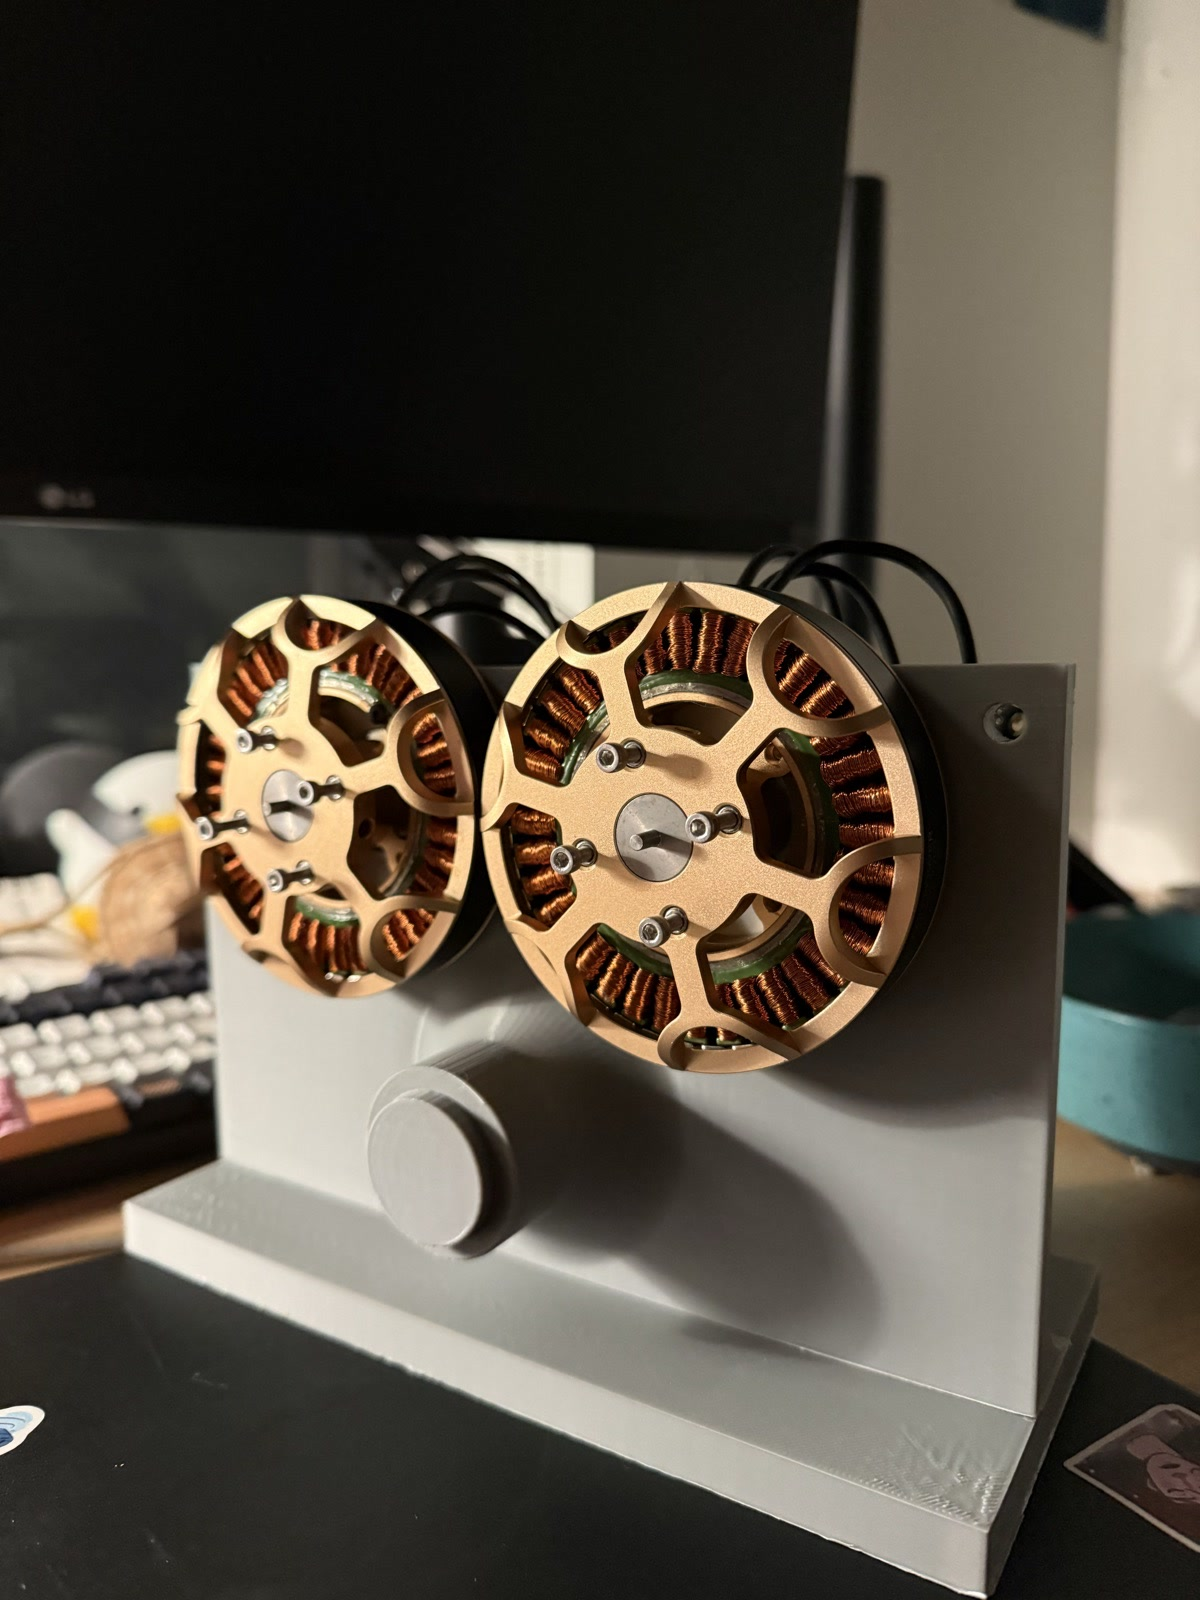
\includegraphics[height=0.4\textheight]{cool_pic_for_profile.jpg}
  \caption{The finished test stand: two EaglePower 8308 BLDC motors mounted
  side by side on a 3D-printed base, each with its own Moteus r4.11 controller
  on the back. The cylindrical boss below the motors is the bearing housing for
  the shared output axle.}
  \label{fig:hero}
\end{figure}

\begin{abstract}
\noindent
With support from the BDW Makers Grant, I designed and built a test stand for a
dual-motor capstan drive, the first subsystem of a 3-degree-of-freedom quadruped
robot leg. Two EaglePower 8308 brushless motors each drive a small
rope-wrapped drum. A 2\,mm Dyneema line couples each small drum to a large
output drum, giving an 8:1 reduction with no gear teeth and therefore no
backlash. The two large drums share an axis but turn independently, so a single
hip location can drive both input links of a planar four-bar leg. I chose the
motor controllers and communication bus, sized the drums from first principles,
went through four iterations of the 3D-printed base, wired and calibrated the
electronics, and reached closed-loop rotation of both motors over a daisy-chained
CAN-FD bus. This report covers the motivation, the design calculations, the
build, the mistakes I made along the way, and what comes next.
\end{abstract}

\tableofcontents
\newpage

% ===============================================================
\section{Motivation}
% ===============================================================

Legged robots need actuators that are strong, fast, and \emph{transparent}: the
motor should be able to feel forces at the foot so the controller can react to
impacts and uneven ground. Conventional gearboxes give torque but add backlash,
friction, and reflected inertia, all of which hide those forces from the motor.
Commercial quasi-direct-drive actuators solve this, but they cost far more than
a student budget.

This project started from three goals:
\begin{enumerate}
  \item \textbf{Use accessible fabrication.} Every structural part is 3D printed,
        so I can make complex geometry at home and change it overnight.
  \item \textbf{Learn mechanisms in depth.} A robot leg brings together power
        transmission, kinematics, bearings, sensing, and embedded control.
  \item \textbf{Iterate quickly.} Printed parts are cheap and modular, so a
        failed design costs a few hours instead of a machining order.
\end{enumerate}

The design draws on two open-source projects: Aaed Musa's capstan drive test
stand and the Stanley capstan-based quadruped kit. Both showed that a printed
capstan reduction can perform close to a commercial actuator. My goal was to go
past copying either design and build a \emph{two-motor, coaxial-output} version
that can drive a full leg. The total budget was about \$500.

% ===============================================================
\section{Background: Why a Capstan Drive?}
% ===============================================================

\subsection{The capstan equation}

A capstan is a rotating drum with a rope wrapped around it. Sailors used them to
haul anchors: a small pull on the free end of the rope holds back a very large
load, because friction between the rope and the drum builds up along the whole
wrap. The relationship is the capstan (Euler--Eytelwein) equation:
\begin{equation}
  T_{\text{load}} = T_{\text{hold}}\, e^{\mu \phi},
  \label{eq:capstan}
\end{equation}
where $T_{\text{load}}$ and $T_{\text{hold}}$ are the rope tensions on the two
sides of the drum, $\mu$ is the coefficient of friction between rope and drum,
and $\phi$ is the total wrap angle in radians.

Because the holding ratio grows \emph{exponentially} with wrap angle, a few turns
of rope are enough to make slip impossible in practice. That lets a capstan
drive act like a pair of gears whose ``teeth'' are friction distributed along
the rope.

\subsection{Capstan vs.\ cycloidal/planetary drives}

Before committing, I compared the capstan drive against the cycloidal and
planetary gearboxes that most hobby quadrupeds use.

\begin{table}[H]
\centering
\caption{Drive mechanism trade-offs considered during planning.}
\label{tab:tradeoff}
\begin{tabularx}{\linewidth}{lXX}
\toprule
 & \textbf{Cycloidal / planetary} & \textbf{Capstan} \\
\midrule
Backlash      & Small but non-zero; grows with wear & Effectively zero when tensioned \\
Smoothness    & Tooth engagement causes ripple       & Continuous rope contact, very smooth \\
Torque density& High, compact                         & Lower; large output drum \\
Reduction     & High ratios in one stage              & Limited per stage ($\sim$5--10:1) \\
Manufacturing & Tight tolerances, hard to print well  & Simple cylinders and helical grooves \\
Maintenance   & Lubrication                           & Rope must be kept under tension \\
Transparency  & Moderate                              & Excellent (low friction, low inertia) \\
\bottomrule
\end{tabularx}
\end{table}

I chose the capstan drive because zero backlash and smooth, back-drivable motion
matter most for a leg that has to sense contact. Its weaknesses (bulk and the
need for tensioning) are acceptable for a test stand and can be designed around
later.

% ===============================================================
\section{System Architecture}
% ===============================================================

\subsection{Leg concept}

The target leg has three degrees of freedom:
\begin{itemize}
  \item \textbf{Two planar DOF (hip and knee):} two motors placed side by side
        each drive one large capstan drum. The large drums are
        \emph{coaxial but independent}, so both inputs of a four-bar linkage
        come out of a single hip point. Offsetting the linkage attachment
        points on the two drums gives two independent motions from one axis of
        rotation.
  \item \textbf{Ab/adduction DOF:} a third motor rotates the whole leg assembly
        sideways for turning and balance.
\end{itemize}
This grant funded the core of the design: the two-motor coaxial capstan stage.

\subsection{Four-bar linkage kinematics}

I picked a four-bar (parallelogram) linkage for the leg because it is a closed
chain, so the foot position comes straight from trigonometry. For a foot target
$(x,y)$ relative to the hip, with upper link length $L_1$ and lower link length
$L_2$:
\begin{align}
  D        &= \sqrt{x^2 + y^2}, &
  \gamma   &= \operatorname{atan2}(y, x), \\
  \alpha   &= \arccos\!\left(\frac{L_1^2 + D^2 - L_2^2}{2 L_1 D}\right), &
  \beta    &= \arccos\!\left(\frac{L_1^2 + L_2^2 - D^2}{2 L_1 L_2}\right), \\
  \theta_1 &= \gamma - \alpha, &
  \theta_2 &= \pi - \beta .
\end{align}
The forward kinematics, used to check the solution, are
\begin{align}
  x &= L_1\cos\theta_1 + L_2\cos(\theta_1+\theta_2), \\
  y &= L_1\sin\theta_1 + L_2\sin(\theta_1+\theta_2).
\end{align}
Each joint angle maps to a motor angle through the drive ratio,
$\phi_{\text{motor}} = N\,\theta_{\text{joint}}$, where $N = 8$ for this drive.

To build intuition before cutting any parts, I wrote an interactive 2-DOF leg
simulator in React/TypeScript (available on my portfolio). It draws the linkage
in SVG, runs foot trajectories in a \texttt{requestAnimationFrame} loop, and
solves inverse kinematics numerically with a two-pass coarse-to-fine grid
search. It also plots the commanded and actual foot paths, which made it easy
to find workspace limits and singular poses.

\subsection{Electronics}

\begin{table}[H]
\centering
\caption{Core electronic components.}
\label{tab:electronics}
\begin{tabularx}{\linewidth}{lX}
\toprule
\textbf{Component} & \textbf{Role / key specs} \\
\midrule
2$\times$ EaglePower 8308 BLDC (90\,KV) & Actuators. 6S--12S input
  (\SIrange{22.2}{44.4}{\volt}), \SI{900}{\watt} max, \SI{22}{\ampere} continuous. \\
2$\times$ mjbots Moteus r4.11 & Field-oriented control (FOC) motor drivers,
  \SIrange{10}{44}{\volt} input, onboard magnetic encoder. \\
mjbots fdcanusb (mjcanfd-usb-1x) & CAN-FD to USB bridge to the host computer. \\
\SI{24}{\volt}, \SI{25}{\ampere} AC--DC supply & Bench power for both controllers. \\
Diametric magnets + printed holders & Rotor position sensing for the encoders. \\
Raspberry Pi (planned) & Onboard host, so the robot can run untethered. \\
\bottomrule
\end{tabularx}
\end{table}

\paragraph{Controller choice: ODrive vs.\ Moteus.}
Aaed Musa's design uses an ODrive S1 (about \$150 per controller). The Stanley
quadruped uses Moteus controllers, and the r4.11 costs about \$59. With a
\$500 budget and at least two (eventually three) motors, the Moteus was the only
choice that fit. It also mounts directly on the back of the motor and reads
rotor position with its onboard encoder, which saves wiring and space.

\paragraph{Why CAN-FD.}
CAN-FD (Controller Area Network with Flexible Data-rate) is a differential,
multi-drop bus built for real-time control in noisy environments. All
controllers share one pair of data lines, each with a unique ID (1 and 2 here).
That gives three benefits:
\begin{itemize}
  \item \textbf{Simple wiring:} controllers are daisy-chained, so there is no
        separate cable from each one back to the host.
  \item \textbf{Scalability:} a full quadruped (12 motors) only means adding
        nodes to the chain.
  \item \textbf{Autonomy later:} the host can be a laptop now and a Raspberry Pi
        on the robot later, with no change to the bus.
\end{itemize}

% ===============================================================
\section{Capstan Drive Design}
% ===============================================================

\begin{figure}[H]
  \centering
  \begin{subfigure}[b]{0.48\linewidth}
    \centering
    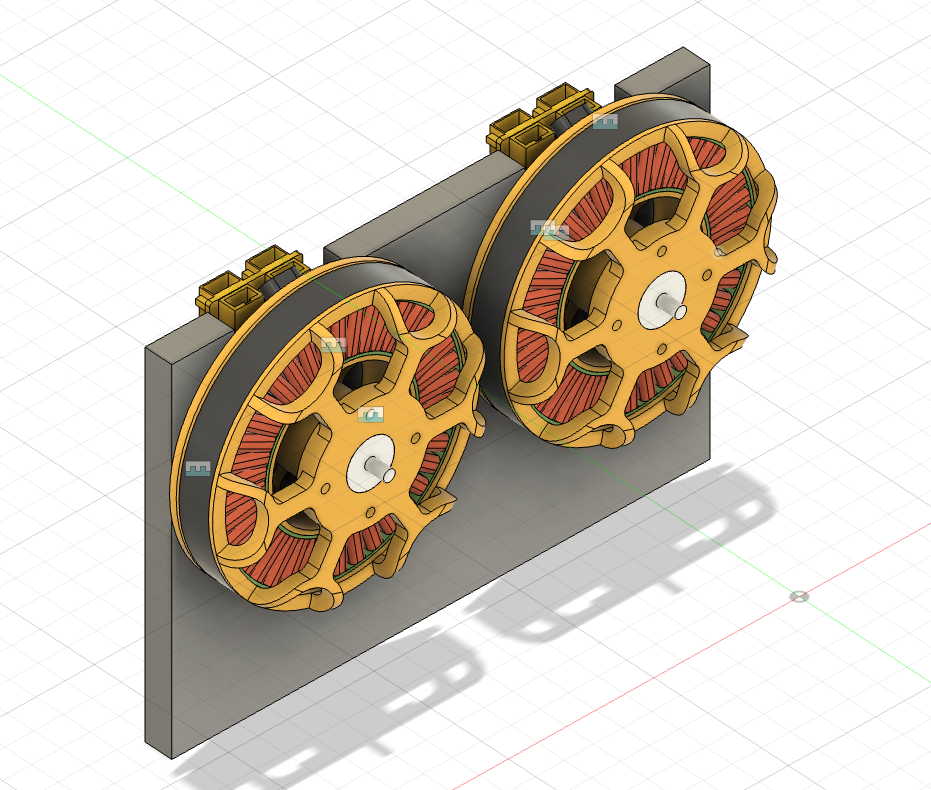
\includegraphics[width=\linewidth]{2_side_by_side.png}
    \caption{Base and dual-motor layout in Fusion 360.}
    \label{fig:cad-layout}
  \end{subfigure}\hfill
  \begin{subfigure}[b]{0.48\linewidth}
    \centering
    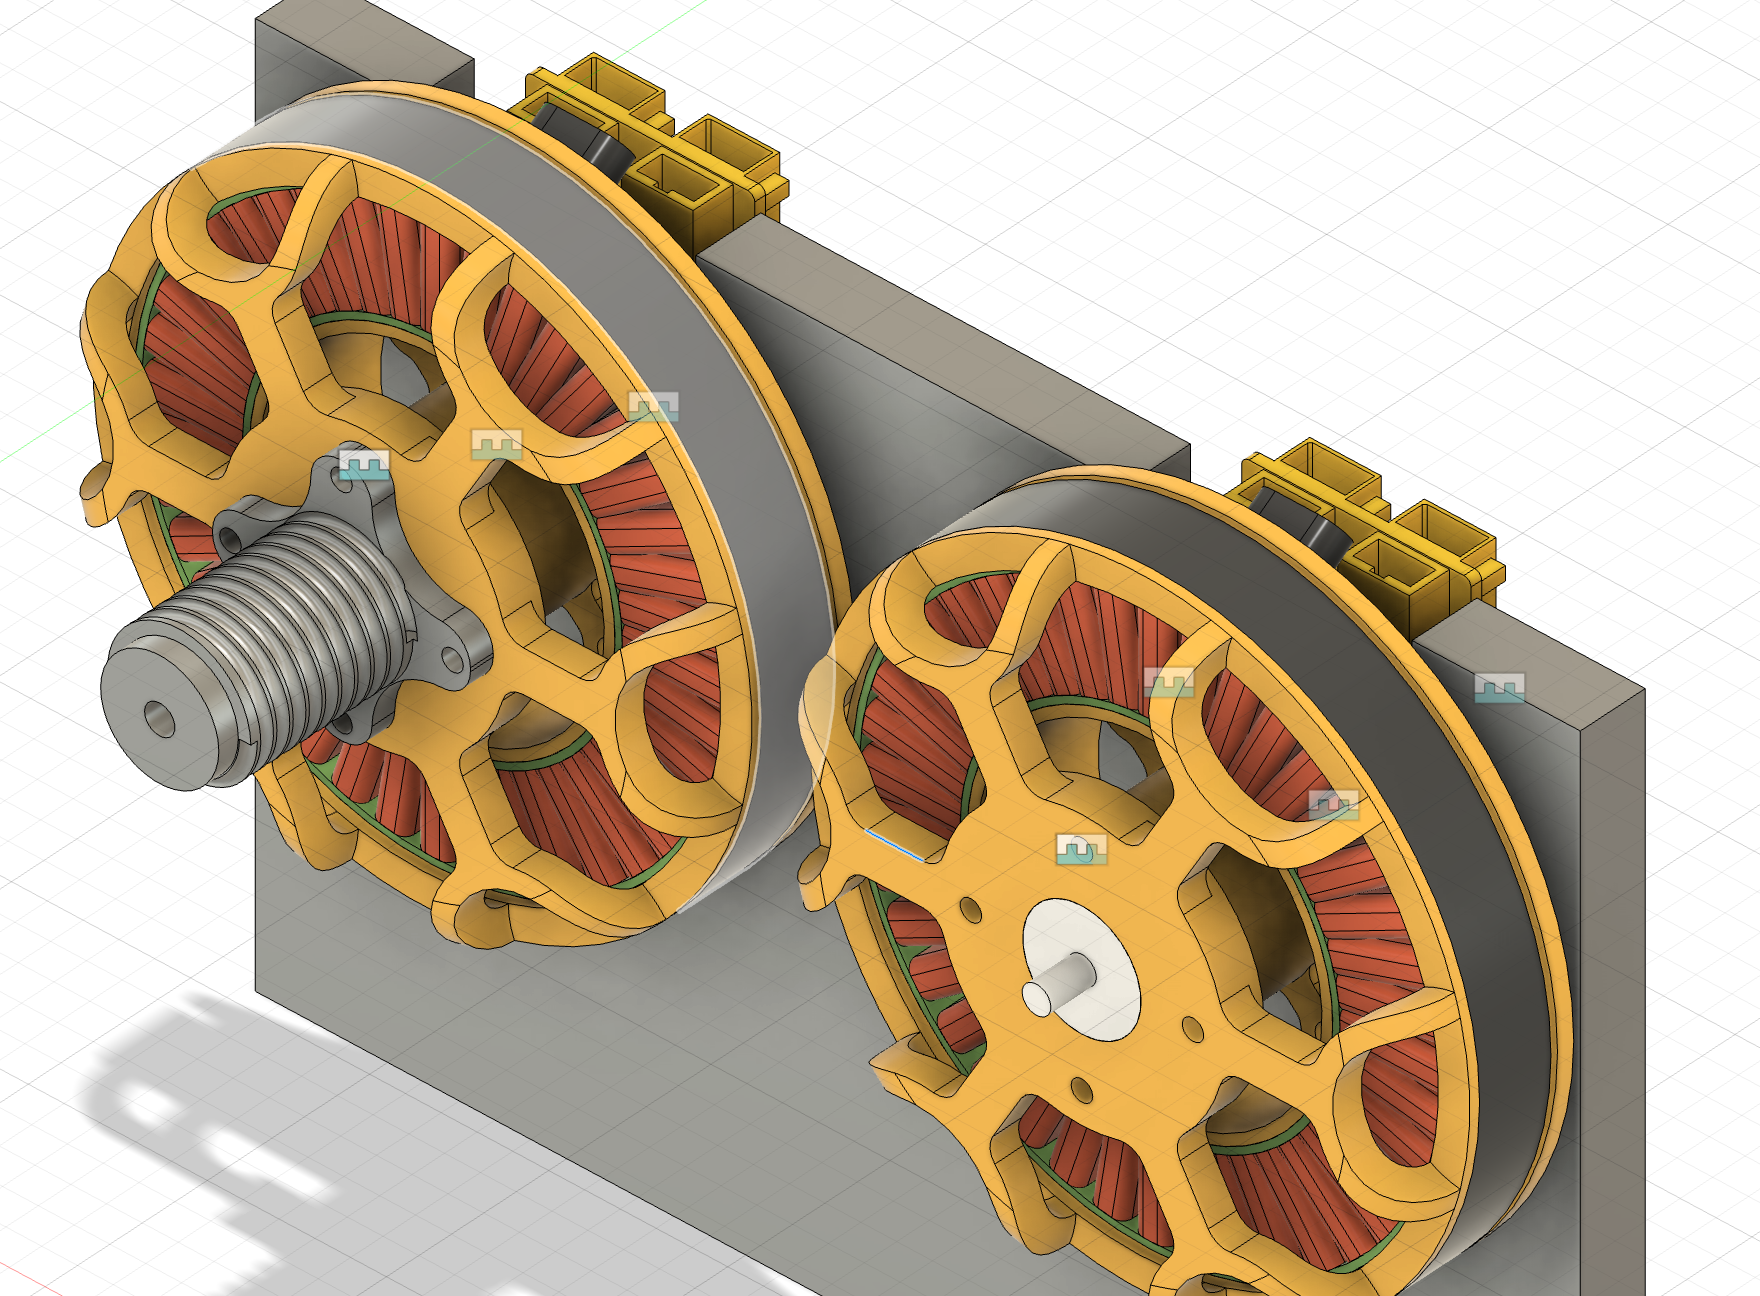
\includegraphics[width=\linewidth]{small_drum.png}
    \caption{Grooved small drum mounted on motor 1.}
    \label{fig:cad-drum}
  \end{subfigure}
  \caption{CAD of the test stand. Each motor carries a small helically grooved
  drum that the Dyneema line wraps around.}
  \label{fig:cad}
\end{figure}

\subsection{Setting the 8:1 ratio with effective diameters}

A capstan drive's reduction comes from the ratio of drum diameters, but the
diameters that count are the \emph{effective} ones: measured at the centerline
of the rope as it lies on each drum, not at the drum surface. Scaling the outer
diameters by eight would give the wrong ratio, because the rope's thickness adds
the same amount to both drums.
\begin{equation}
  N = \frac{D_{\text{eff,large}}}{D_{\text{eff,small}}}.
\end{equation}

\begin{table}[H]
\centering
\caption{Drum geometry.}
\label{tab:drums}
\begin{tabular}{lcc}
\toprule
 & \textbf{Small drum} & \textbf{Large drum} \\
\midrule
Effective diameter (rope centerline) & \SI{18}{\milli\metre} & \SI{144}{\milli\metre} \\
Outer diameter                        & \SI{20}{\milli\metre} & \SI{146}{\milli\metre} \\
Groove coil diameter                  & \SI{19}{\milli\metre} & \SI{145}{\milli\metre} \\
Groove profile (circular section)     & \SI{2.2}{\milli\metre} & \SI{2.2}{\milli\metre} \\
Pitch / turns / height & \multicolumn{2}{c}{\SI{2.5}{\milli\metre} / 10 / \SI{25}{\milli\metre}} \\
\midrule
Reduction & \multicolumn{2}{c}{$144 / 18 = 8:1$} \\
\bottomrule
\end{tabular}
\end{table}

\paragraph{Bend ratio.} Synthetic ropes lose strength and wear quickly when bent
around too small a radius. The small drum's \SI{20}{\milli\metre} outer
diameter against the \SI{2}{\milli\metre} Dyneema line gives $D/d = 10$, which
is acceptable for Dyneema and was the limit that set the small drum size. Once
the small drum is fixed, the 8:1 ratio fixes the large drum.

\paragraph{Grooves.} Both drums have helical grooves so the rope lays down
neatly and unwinds in a guided way instead of stacking or walking along the
drum. In Fusion 360 I modeled each groove with the \emph{Coil} tool (10
revolutions over \SI{25}{\milli\metre}, so a \SI{2.5}{\milli\metre} pitch, and a
\SI{2.2}{\milli\metre} circular section that leaves clearance for the
\SI{2}{\milli\metre} rope) and subtracted it from the drum with a
\emph{Combine--Cut}. Figure~\ref{fig:drum-evolution} shows the drum before and
after.

\begin{figure}[H]
  \centering
  \begin{subfigure}[b]{0.42\linewidth}
    \centering
    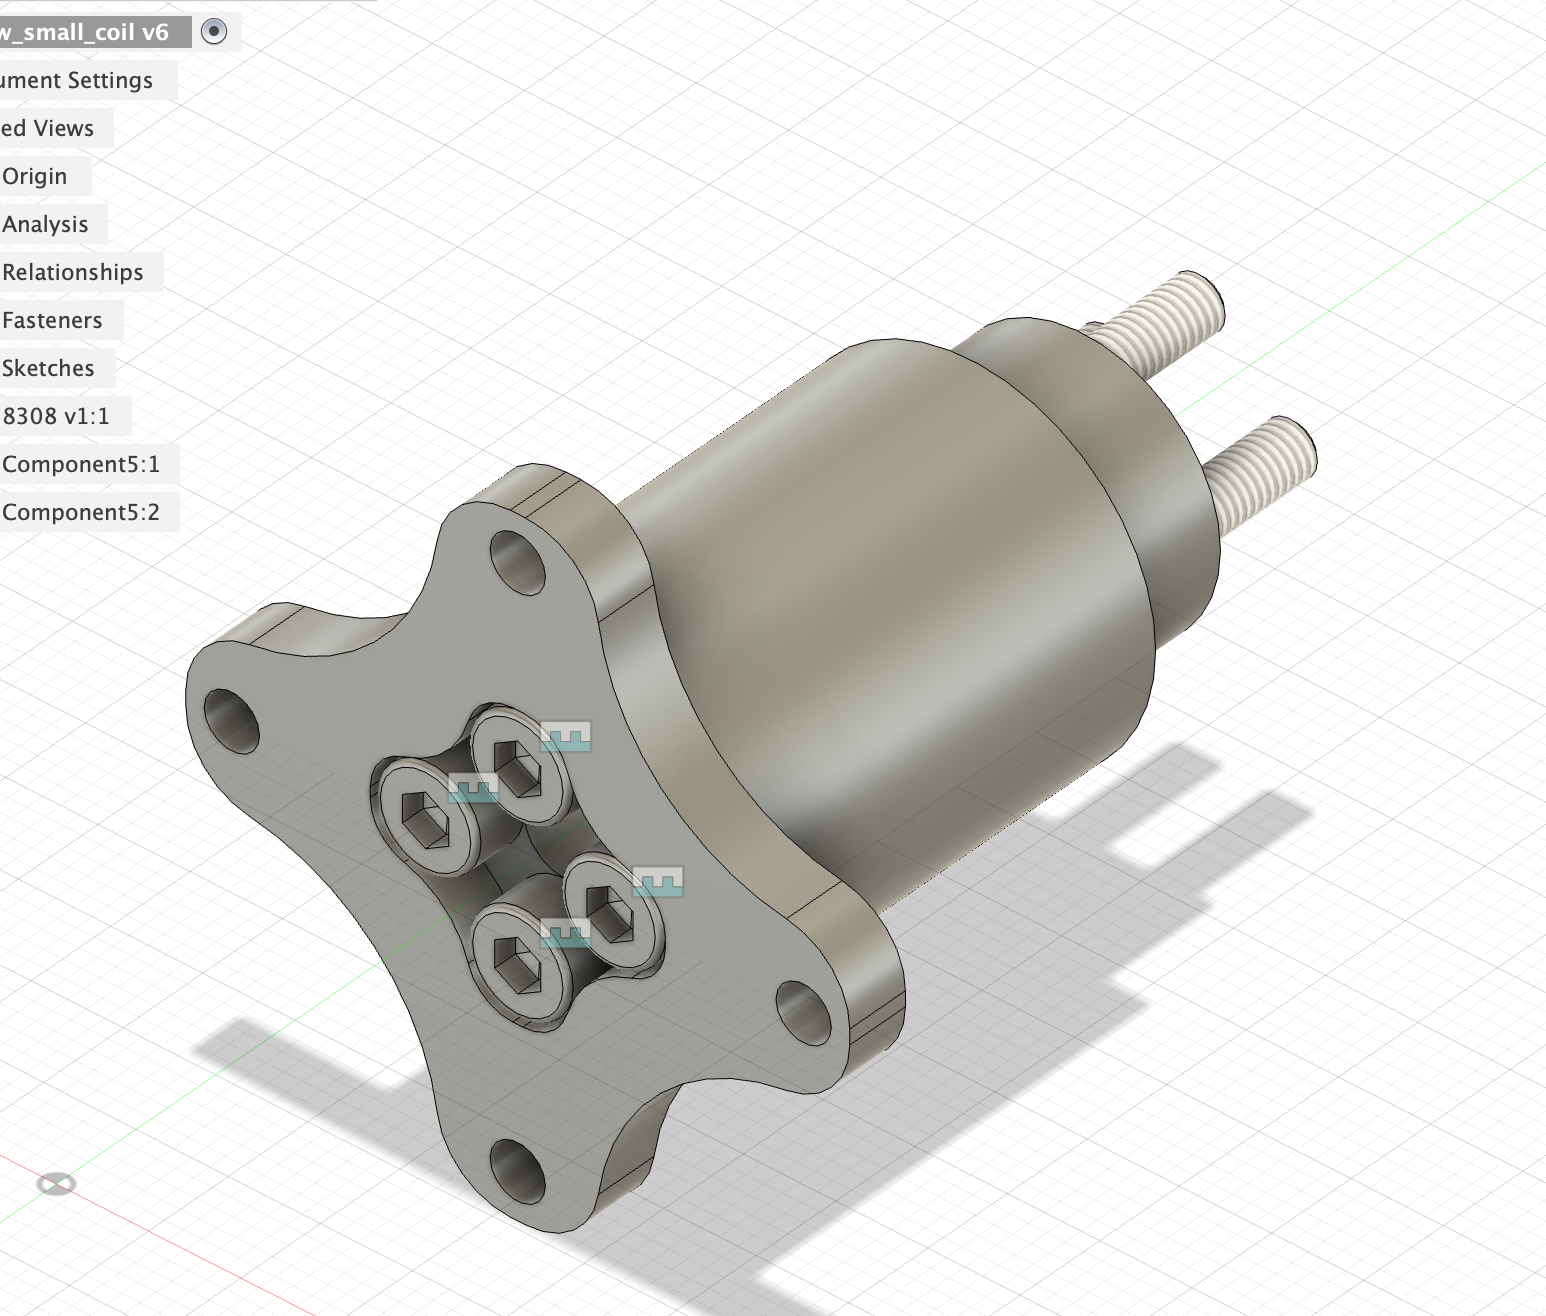
\includegraphics[width=\linewidth]{small_drum_without_grooves.png}
    \caption{Plain drum and motor-adapter flange.}
  \end{subfigure}\hfill
  \begin{subfigure}[b]{0.54\linewidth}
    \centering
    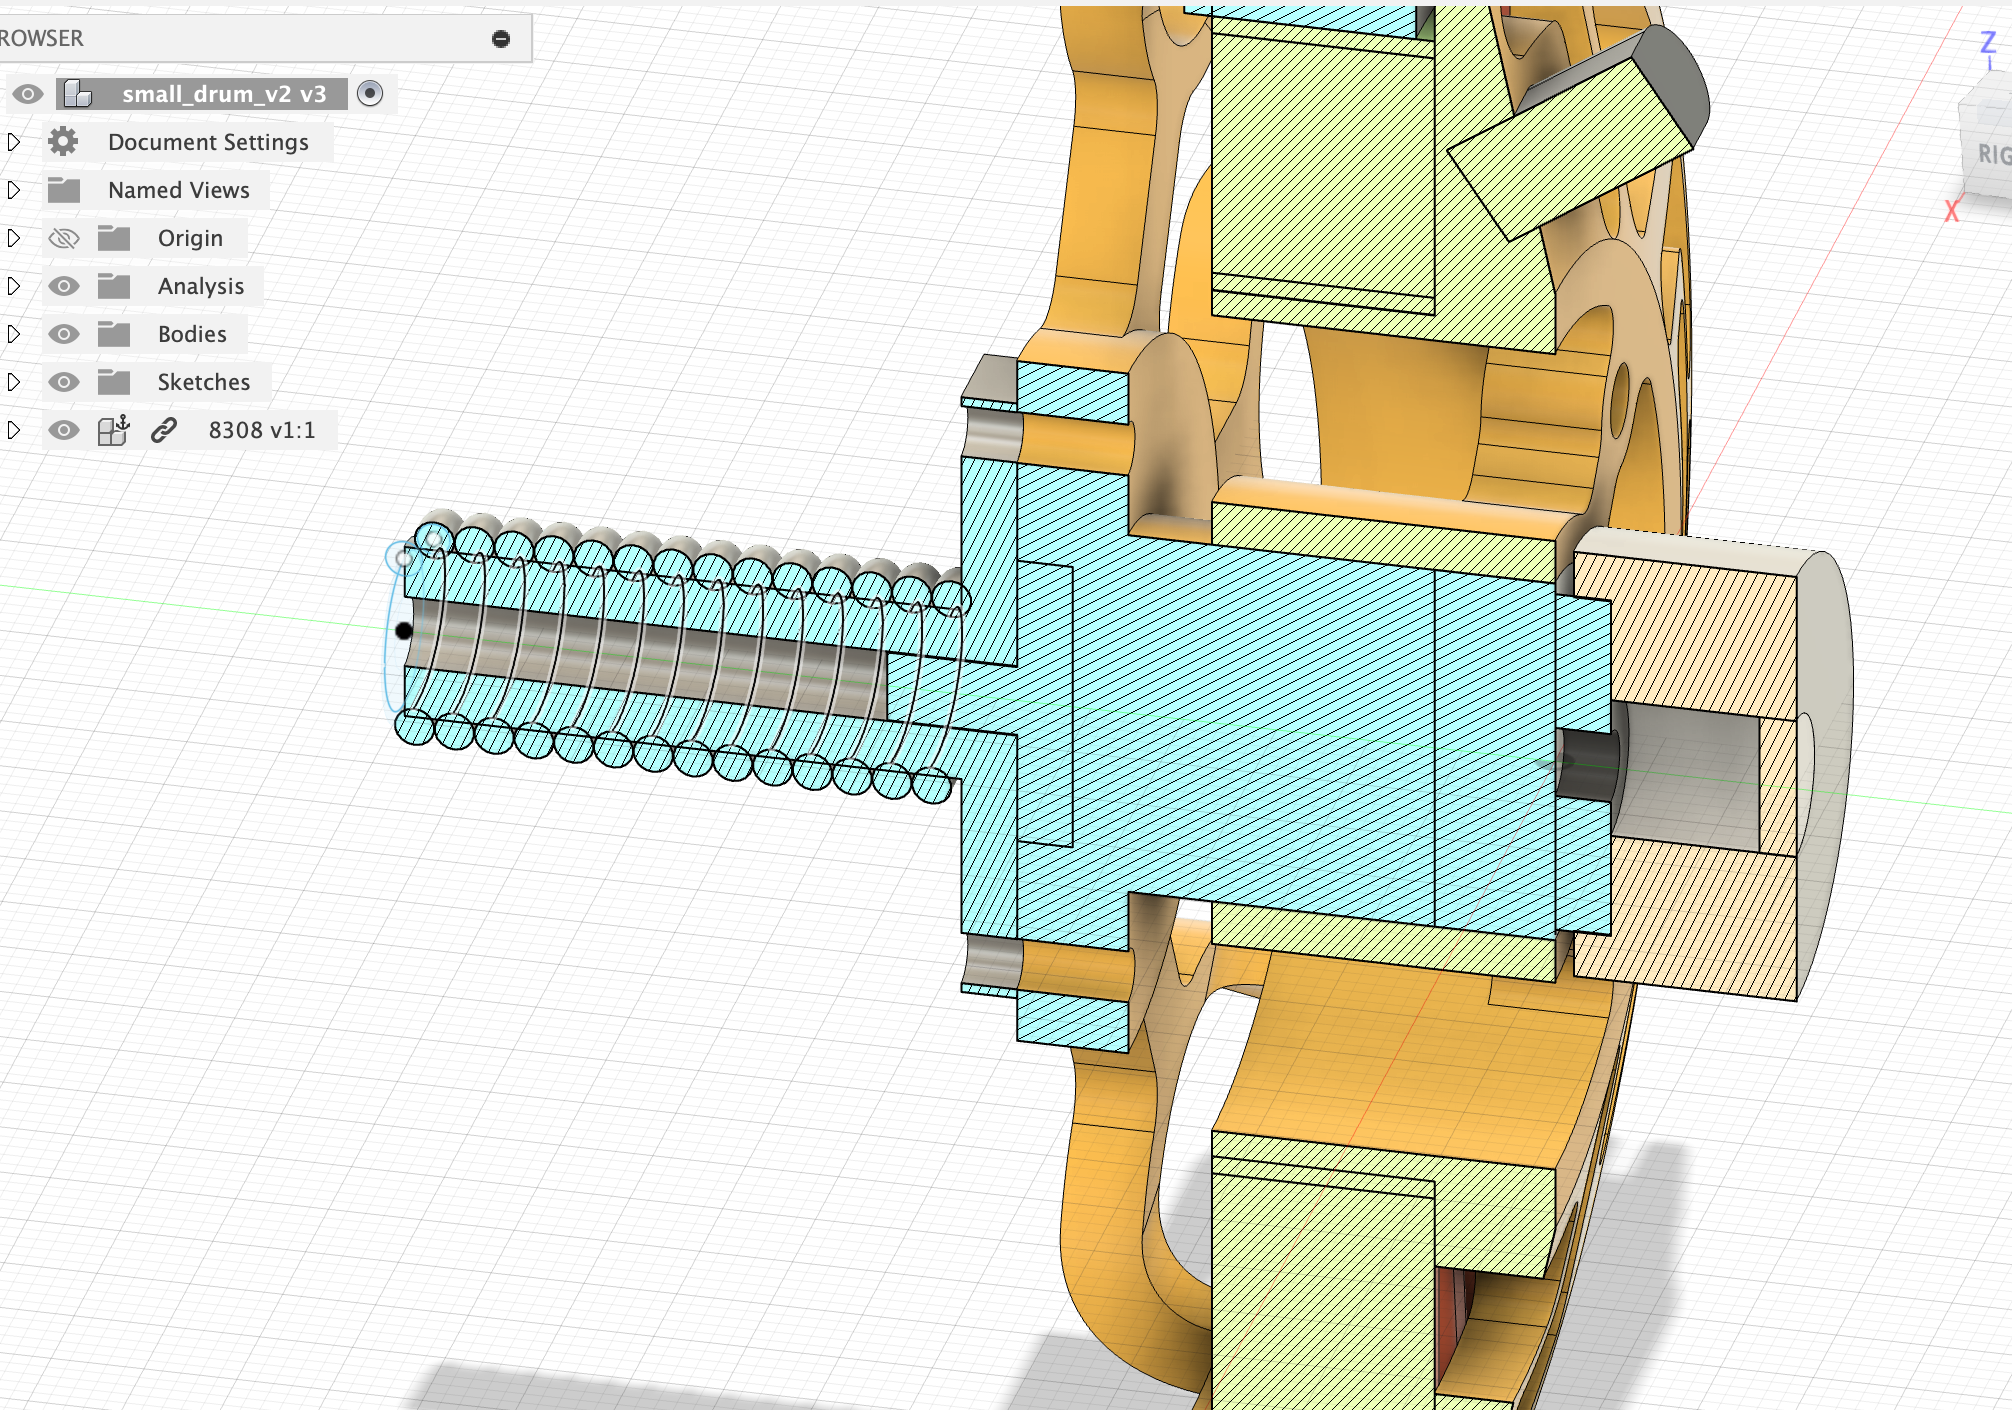
\includegraphics[width=\linewidth]{sectional_analysis_old.png}
    \caption{Section view of the drum on the motor rotor.}
    \label{fig:section}
  \end{subfigure}
  \caption{Small drum development. The section view (b) was used to check how
  the drum adapter, its bolts, and the rotor fit together before printing.}
  \label{fig:drum-evolution}
\end{figure}

\subsection{Slip margin}

With $\mu \approx 0.2$ for Dyneema on PLA and ten full wraps
($\phi = 10 \times 2\pi \approx \SI{62.8}{\radian}$),
equation~\eqref{eq:capstan} gives
\begin{equation}
  \frac{T_{\text{load}}}{T_{\text{hold}}} = e^{0.2 \times 62.8} \approx e^{12.6}
  \approx 2.9 \times 10^{5}.
\end{equation}
In operation only part of the wrap is in contact at once, so the real margin is
smaller. Even so, a few wraps already give a ratio in the hundreds, so slip is
not a realistic failure mode. Note that the number of wraps and the reduction
ratio are \emph{independent}: I mixed them up early on. The ratio comes only
from the diameters. The wraps come from drum height and groove pitch and only
set grip and contact area.

\subsection{Expected output performance}

Using the motor data in Table~\ref{tab:electronics}, a first-order estimate of
the drive output (ignoring rope and bearing losses) is:
\begin{itemize}
  \item \textbf{Torque constant:} $K_t \approx 8.27/K_V = 8.27/90 \approx
        \SI{0.092}{\newton\metre\per\ampere}$.
  \item \textbf{Continuous output torque:} $\SI{0.092}{} \times \SI{22}{\ampere}
        \times 8 \approx \SI{16}{\newton\metre}$ at the large drum.
  \item \textbf{No-load output speed at \SI{24}{\volt}:}
        $90 \times 24 / 8 \approx \SI{270}{rpm}$.
  \item \textbf{Rope tension at that torque:}
        $\SI{16}{\newton\metre} / \SI{0.072}{\metre} \approx \SI{220}{\newton}$,
        far below the breaking strength of \SI{2}{\milli\metre} Dyneema
        (several kilonewtons).
\end{itemize}
The 8:1 ratio keeps the drive \emph{quasi-direct}: high enough to multiply
torque and low enough that the leg stays back-drivable and the motor current
remains a good proxy for foot force.

% ===============================================================
\section{Mechanical Design Iterations}
% ===============================================================

The first layout put two motors on a flat plate. A major revision on 14~November
reorganized the base around the coaxial output: it now carries the coaxial drum
plus a ``through'' drum and an axial drum that supports the through-axle, so the
two output drums share an axis while turning independently.

The base went through \textbf{four printed iterations}. The main changes:
\begin{itemize}
  \item \textbf{Bearings:} 15$\times$28$\times$7\,mm bearings for the small
        drum shafts and 42$\times$50$\times$12\,mm thin-section bearings for
        the large coaxial axle.
  \item \textbf{Fasteners:} heat-set inserts with M2.5 screws for the Moteus
        boards (so they can be removed repeatedly without wearing out the
        plastic), and M3 screws for everything else.
  \item \textbf{Encoder magnet holder:} a dedicated printed holder keeps the
        diametric magnet centered on the motor axis behind each controller.
  \item \textbf{Controller placement:} the Moteus mounting holes were in the
        wrong place on an earlier base. This version fixes that so the onboard
        encoder sits directly over the magnet.
\end{itemize}

\begin{figure}[H]
  \centering
  \begin{subfigure}[b]{0.48\linewidth}
    \centering
    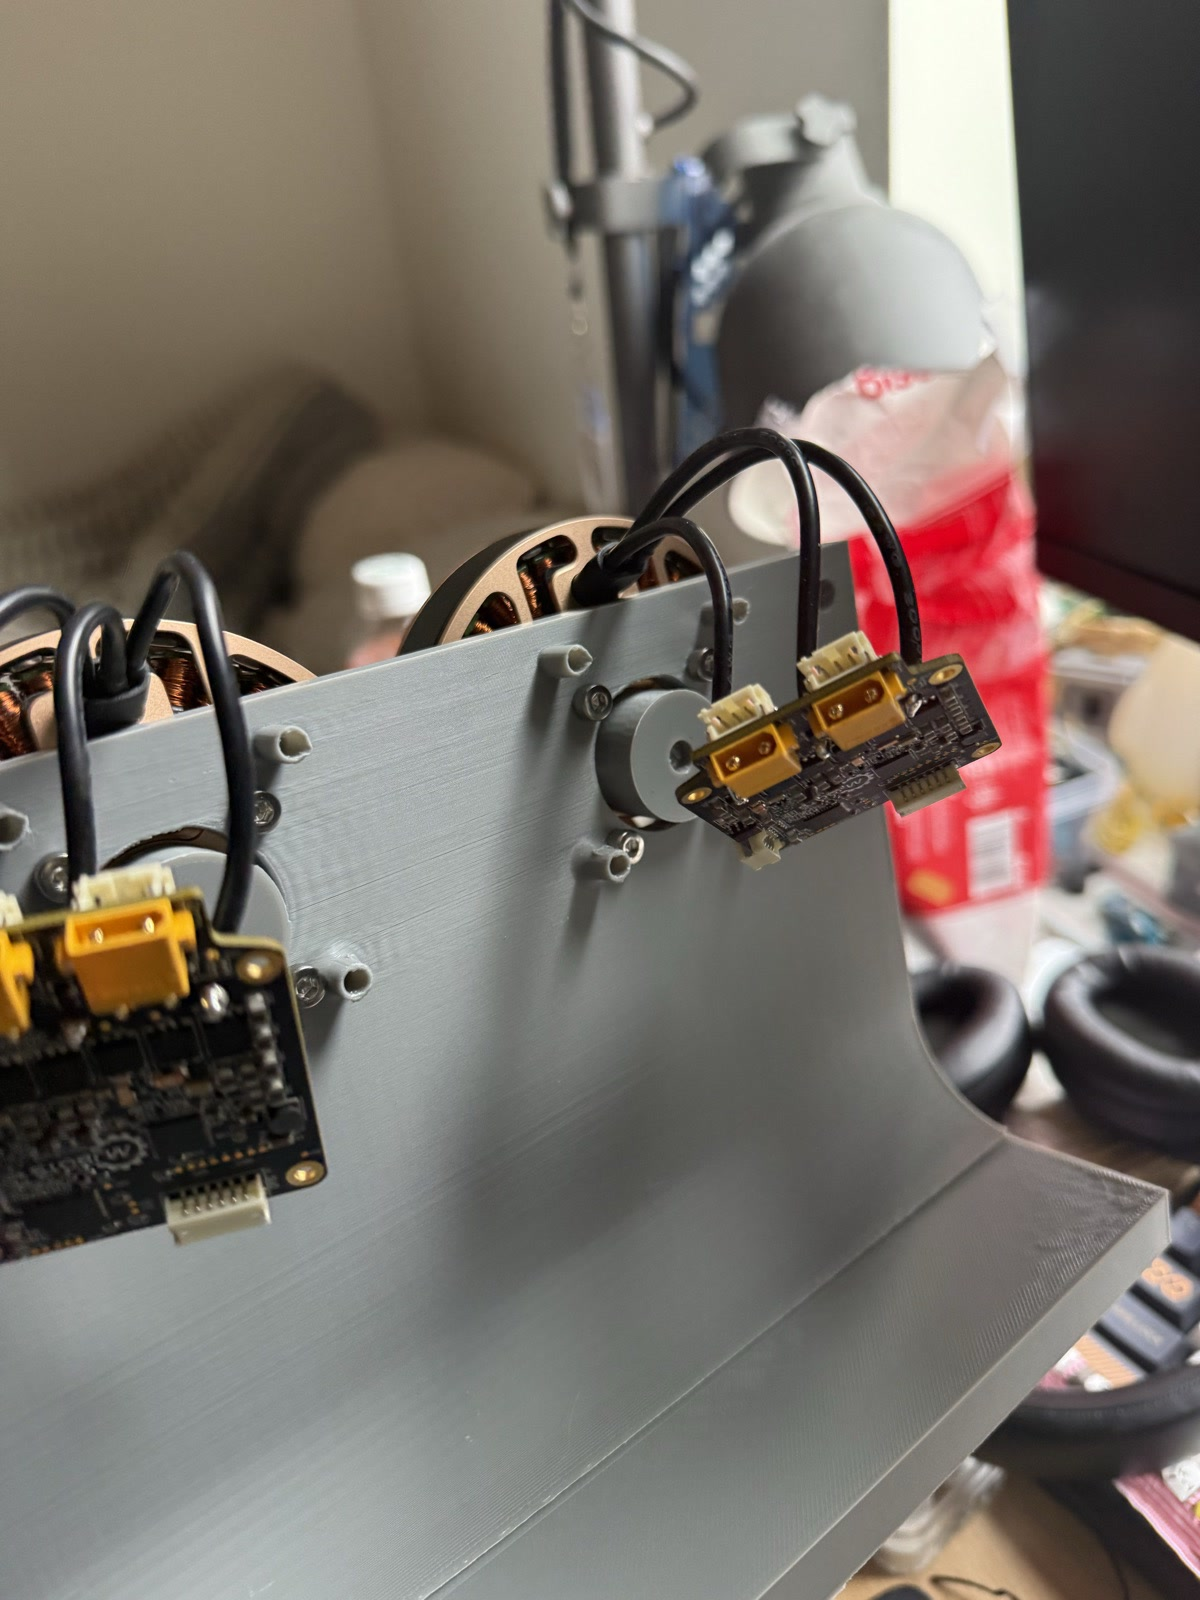
\includegraphics[height=7.5cm]{back_encoder_magnet.jpg}
    \caption{Back of the base with both Moteus r4.11 boards mounted on
    heat-set inserts over the encoder magnets.}
    \label{fig:back}
  \end{subfigure}\hfill
  \begin{subfigure}[b]{0.48\linewidth}
    \centering
    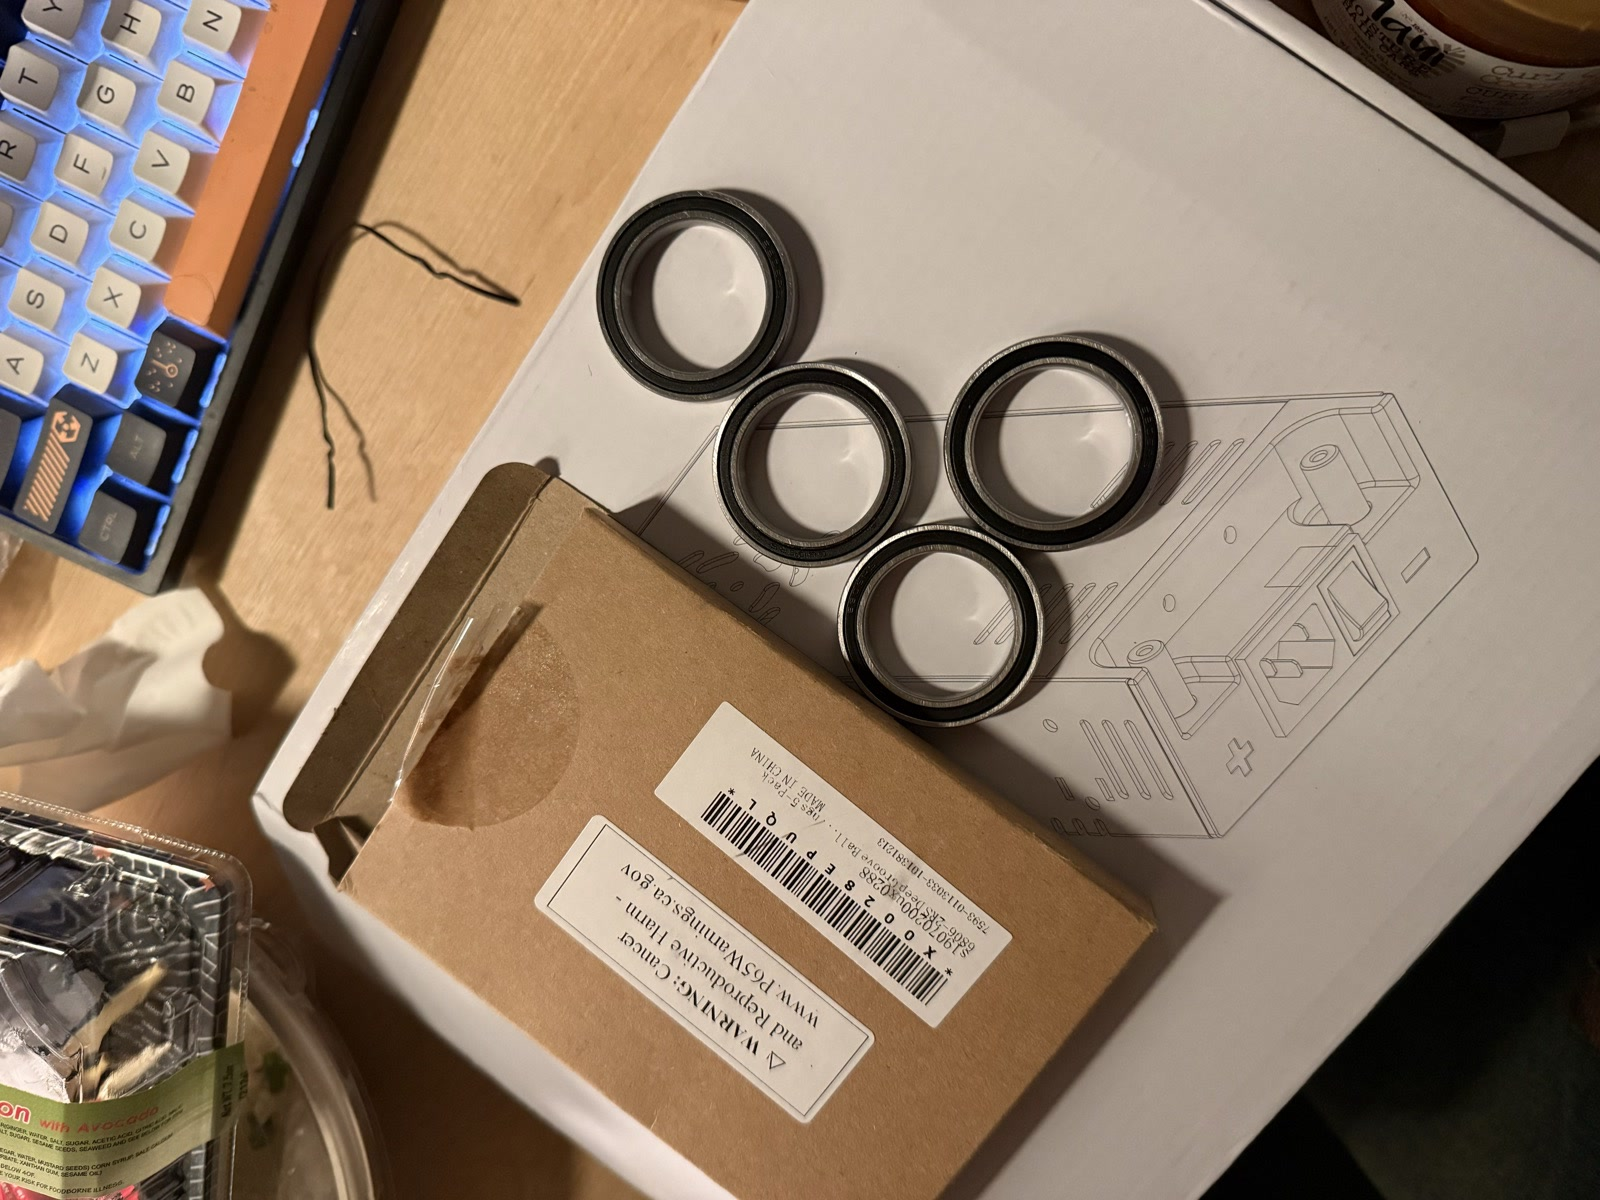
\includegraphics[width=\linewidth]{bearings.jpg}\vspace{1.4cm}
    \caption{Thin-section bearings for the coaxial output axle.}
    \label{fig:bearings}
  \end{subfigure}
  \caption{Printed base and bearings.}
\end{figure}

% ===============================================================
\section{Build and Bring-Up}
% ===============================================================

\subsection{Assembly}

All parts arrived in early November. After the base was printed, I screwed in
the motors and controllers, pressed in the encoder magnets, and soldered XT30
connectors to the power leads (Figure~\ref{fig:assembly}).

\begin{figure}[H]
  \centering
  \begin{subfigure}[b]{0.48\linewidth}
    \centering
    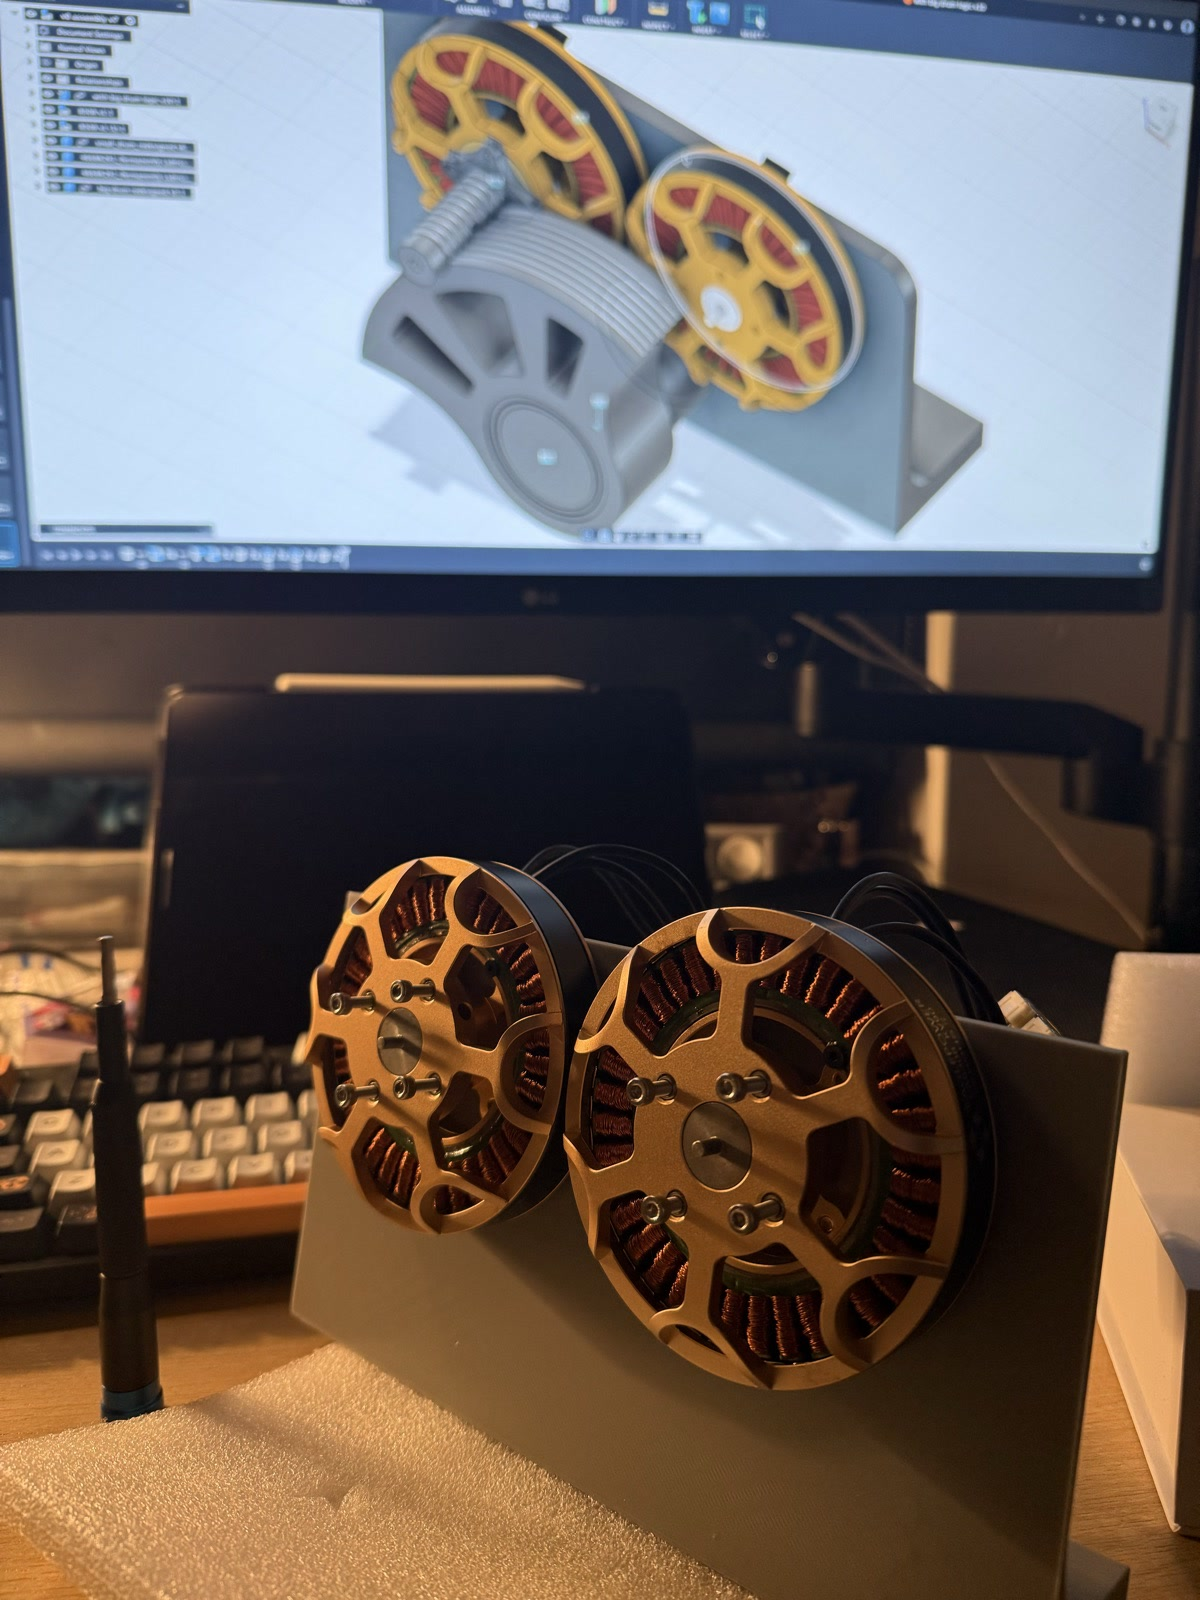
\includegraphics[height=7.5cm]{screwed_into_base.jpg}
    \caption{Motors mounted on the printed base, next to the CAD model.}
  \end{subfigure}\hfill
  \begin{subfigure}[b]{0.48\linewidth}
    \centering
    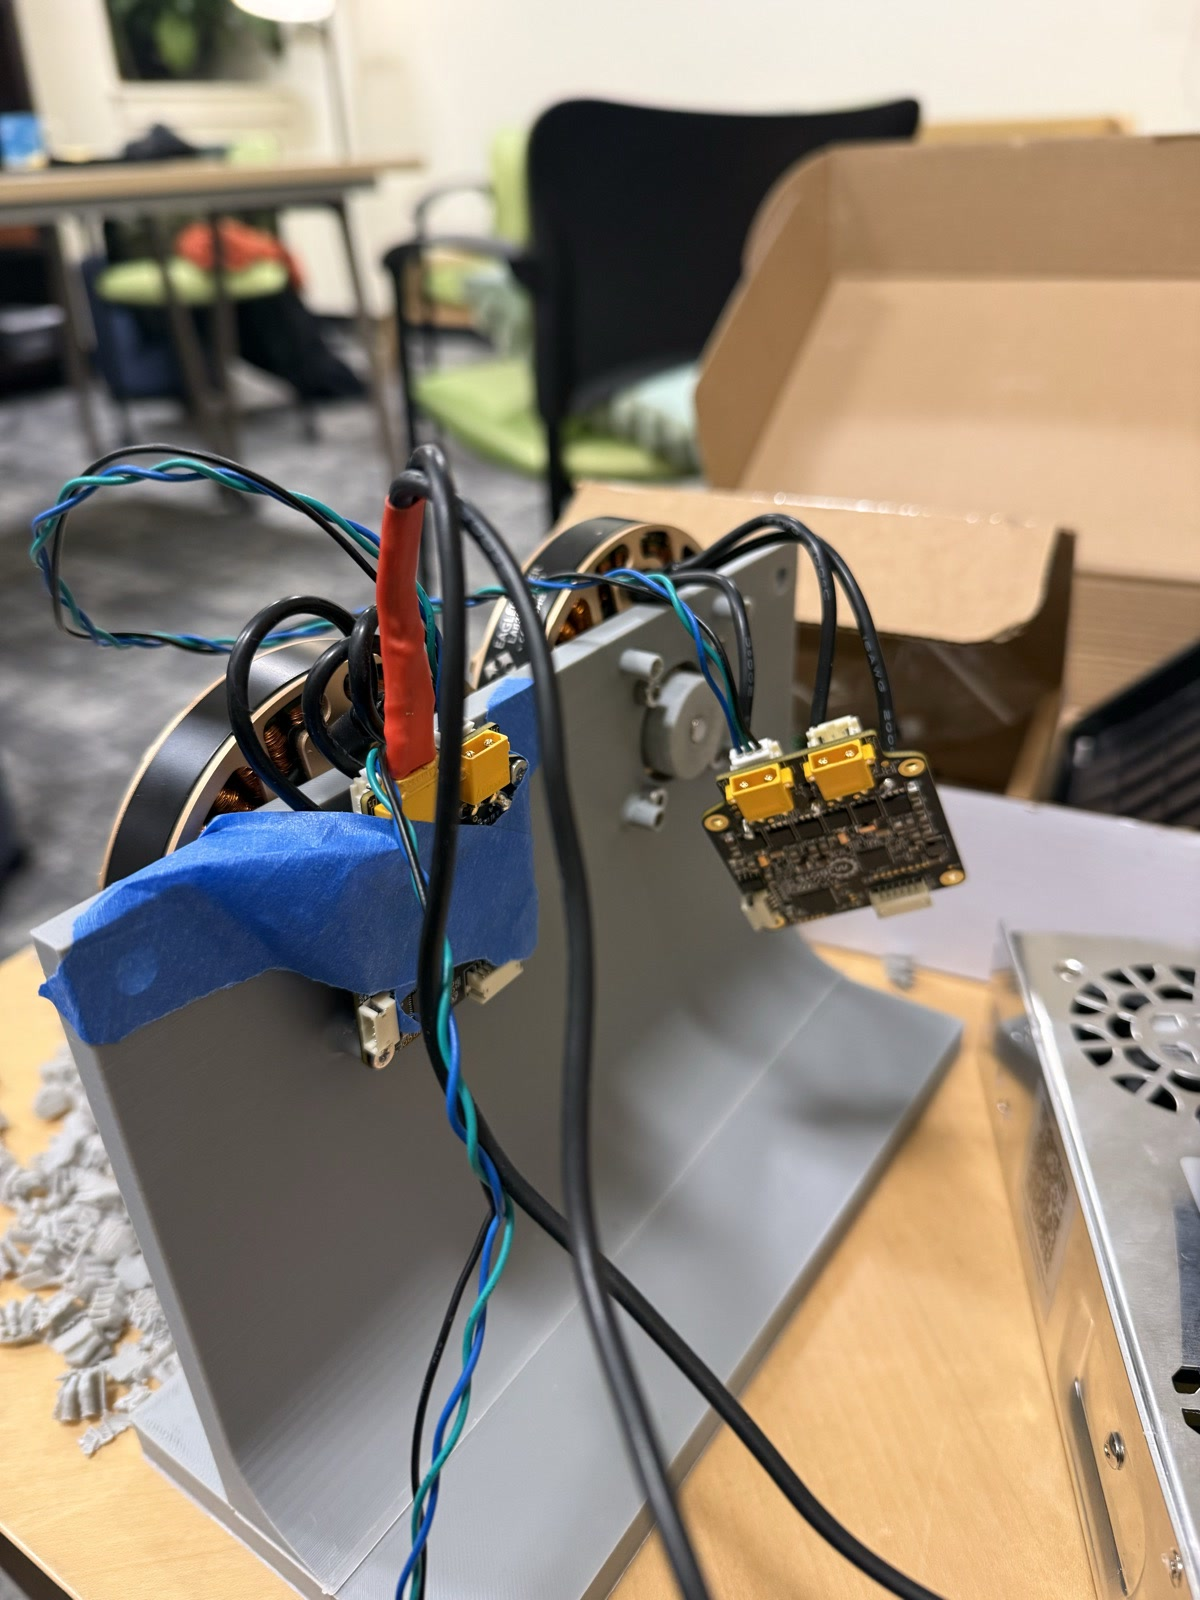
\includegraphics[height=7.5cm]{back.jpg}
    \caption{Power and CAN wiring on the back of the stand.}
  \end{subfigure}
  \caption{Assembly of the test stand.}
  \label{fig:assembly}
\end{figure}

\subsection{First power-on and calibration}

On the first power-on I reversed the supply polarity and the board began to
smoke. I cut power immediately. With the polarity corrected, the controller
came up and its status LED blinked normally. The first calibration then failed
because of a bad configuration. After fixing it, with help from Josh Pieper (the
Moteus developer) on the mjbots Discord, the motor completed calibration and
spun under closed-loop control for the first time on 23~November
(Figures~\ref{fig:first-power}--\ref{fig:spin}).

\begin{figure}[H]
  \centering
  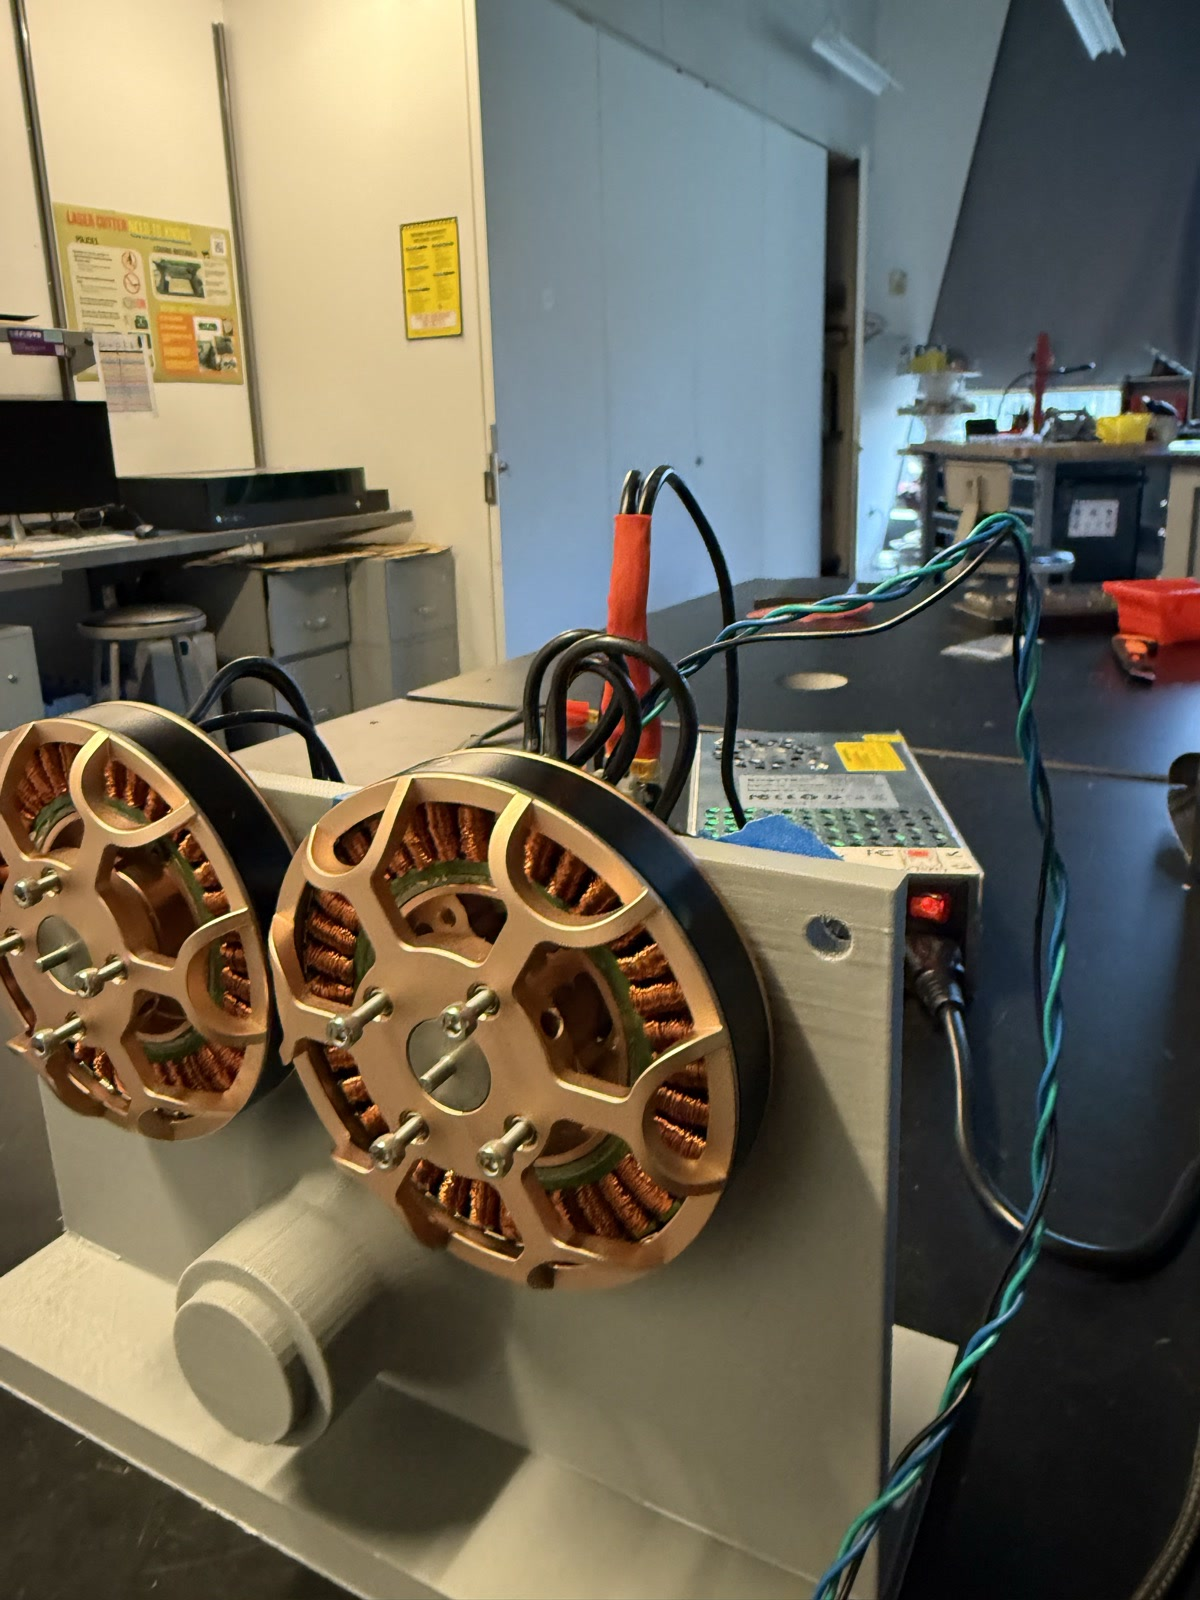
\includegraphics[height=7cm]{first_power.jpg}
  \caption{Both motors and controllers wired to the \SI{24}{\volt} supply for
  the first power-on.}
  \label{fig:first-power}
\end{figure}

\begin{figure}[H]
  \centering
  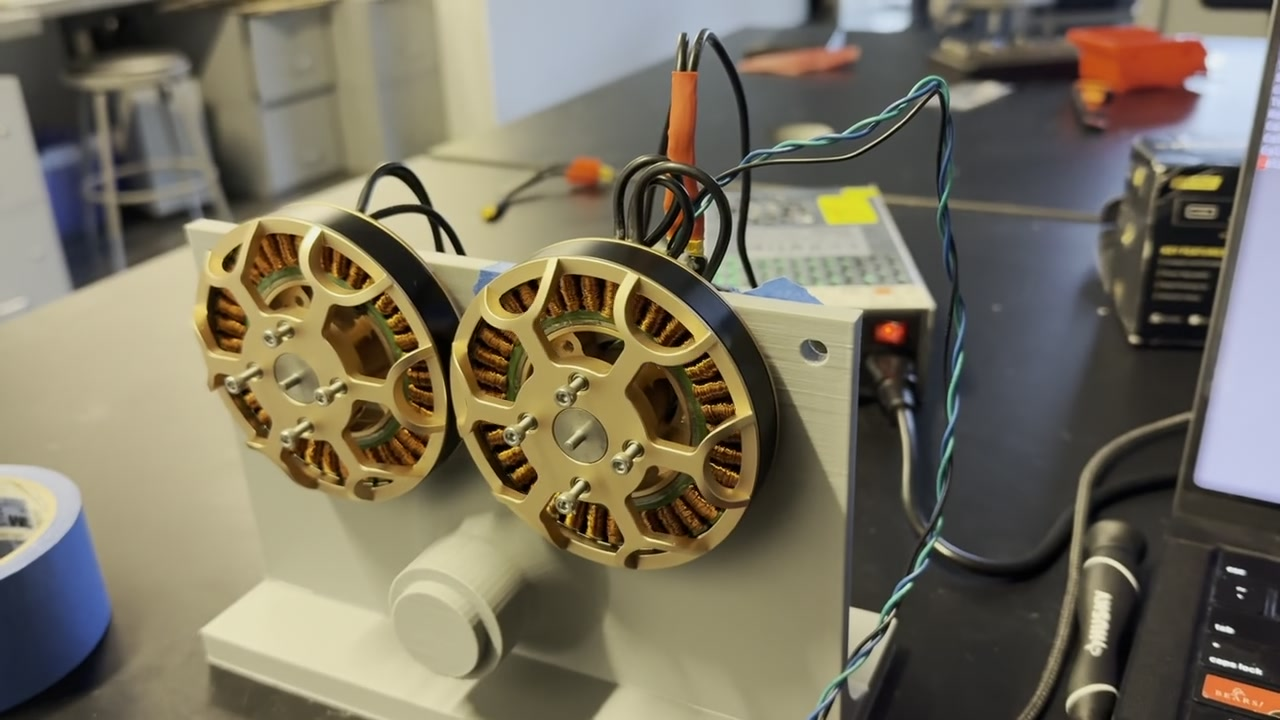
\includegraphics[width=0.8\linewidth]{calibration.jpg}
  \caption{Frame from the calibration video. During calibration the Moteus
  steps the motor through electrical cycles to measure the encoder offset,
  pole count, phase resistance and inductance.}
  \label{fig:calibration}
\end{figure}

\begin{figure}[H]
  \centering
  \begin{subfigure}[b]{0.32\linewidth}
    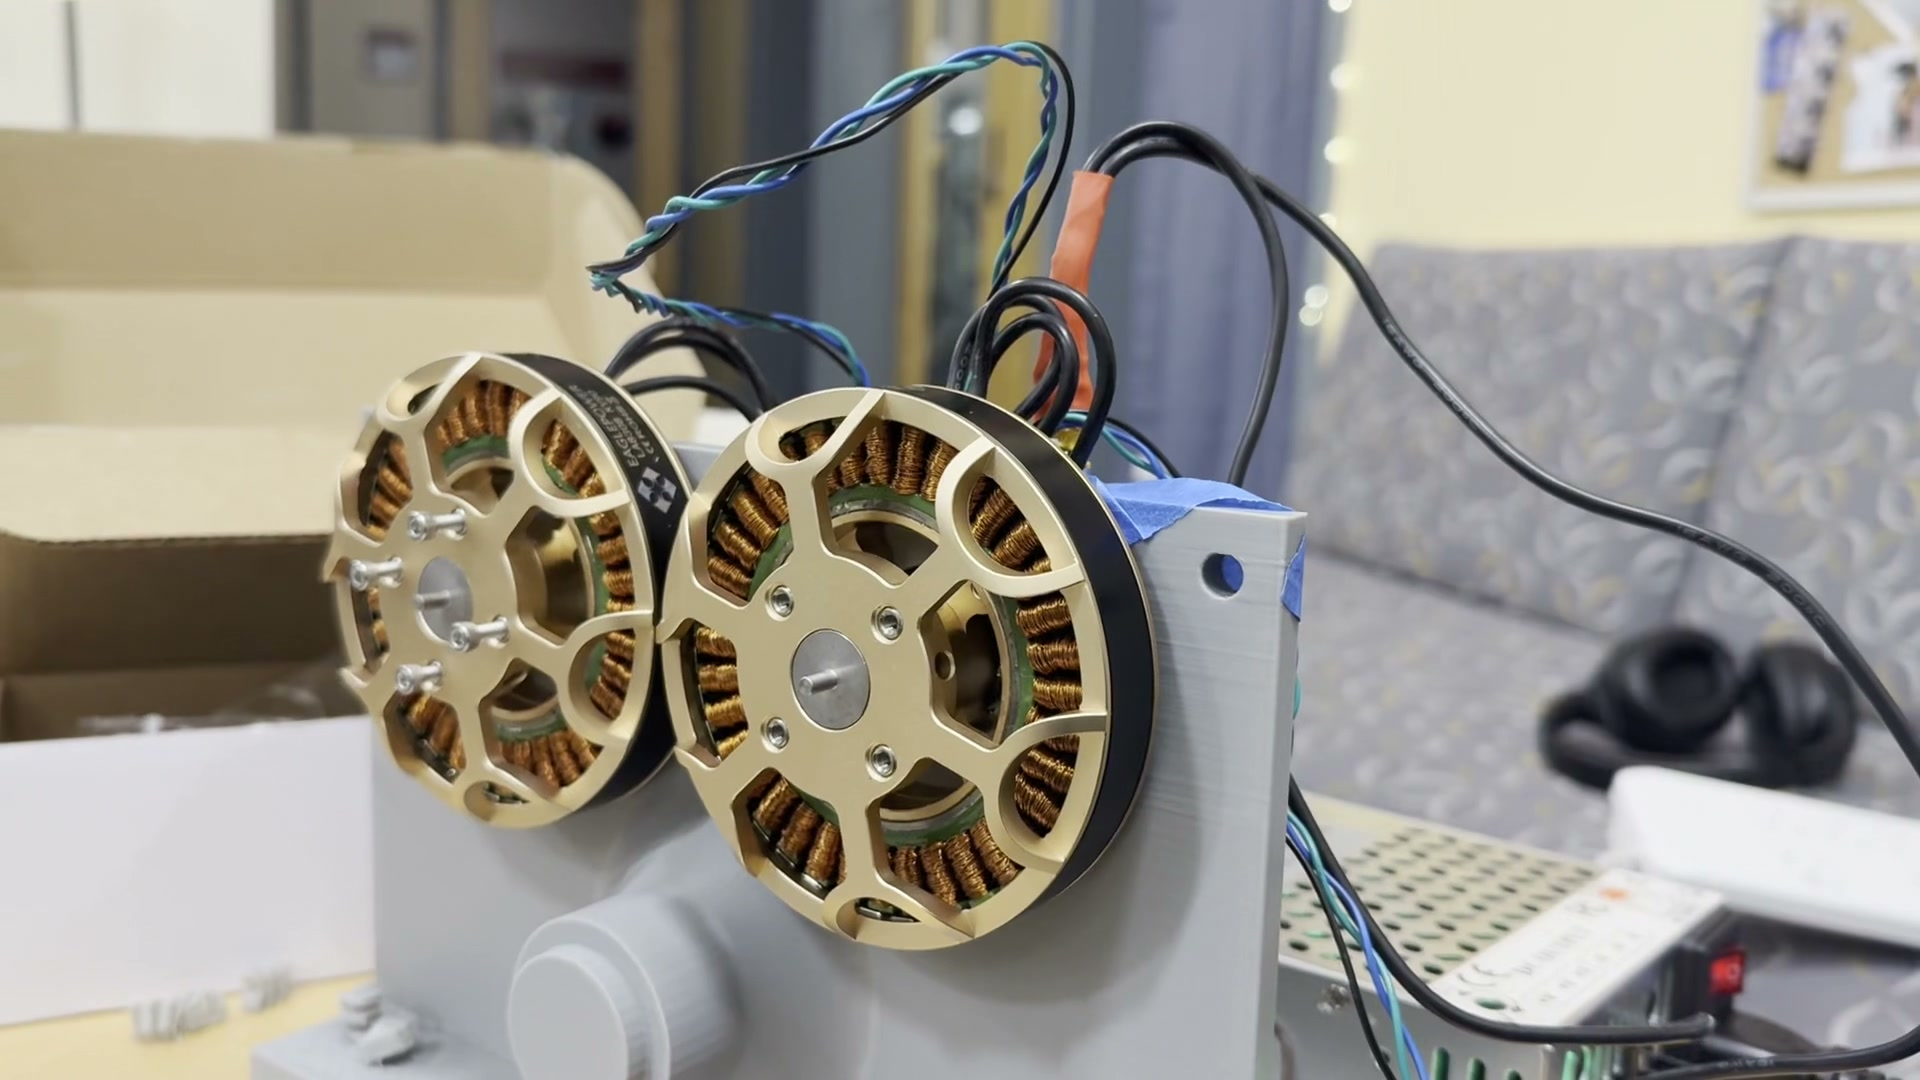
\includegraphics[width=\linewidth]{spin_rest.jpg}
    \caption{At rest.}
  \end{subfigure}\hfill
  \begin{subfigure}[b]{0.32\linewidth}
    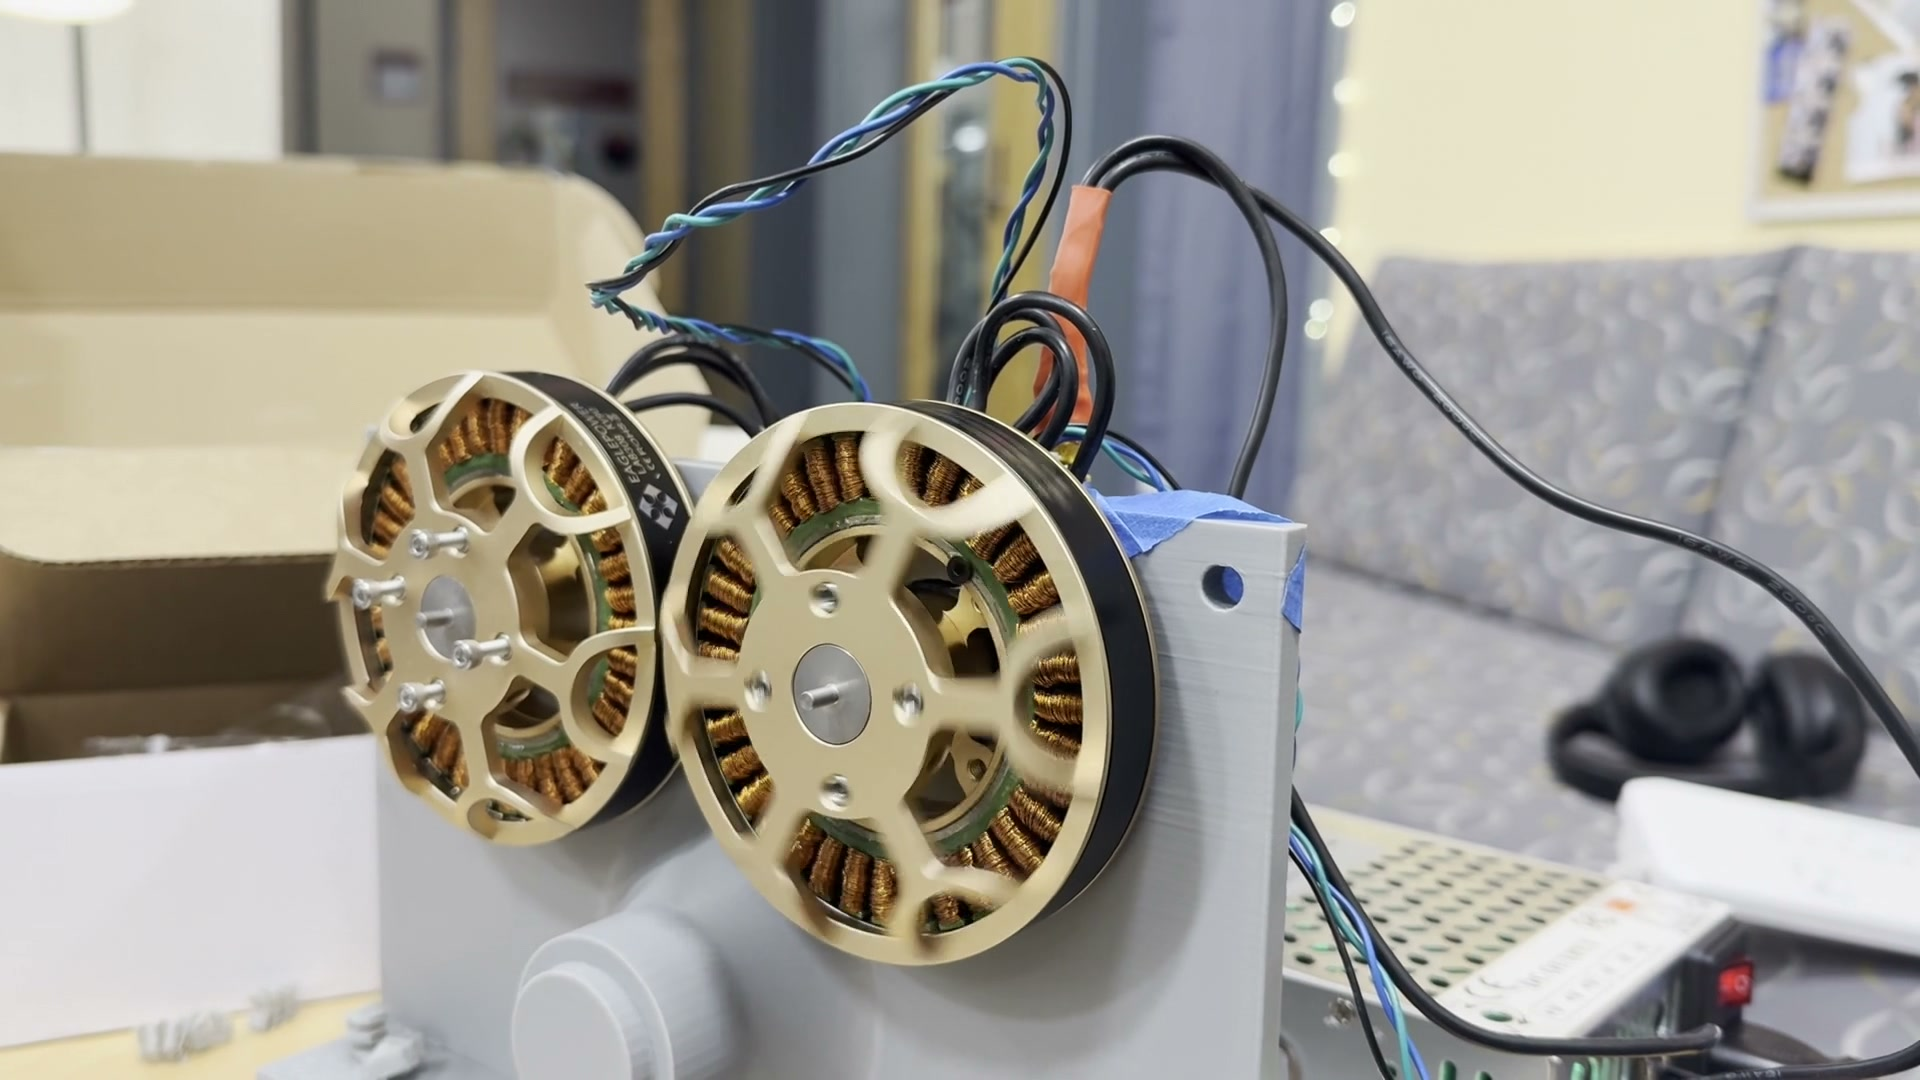
\includegraphics[width=\linewidth]{spin_blur.jpg}
    \caption{Spinning up.}
  \end{subfigure}\hfill
  \begin{subfigure}[b]{0.32\linewidth}
    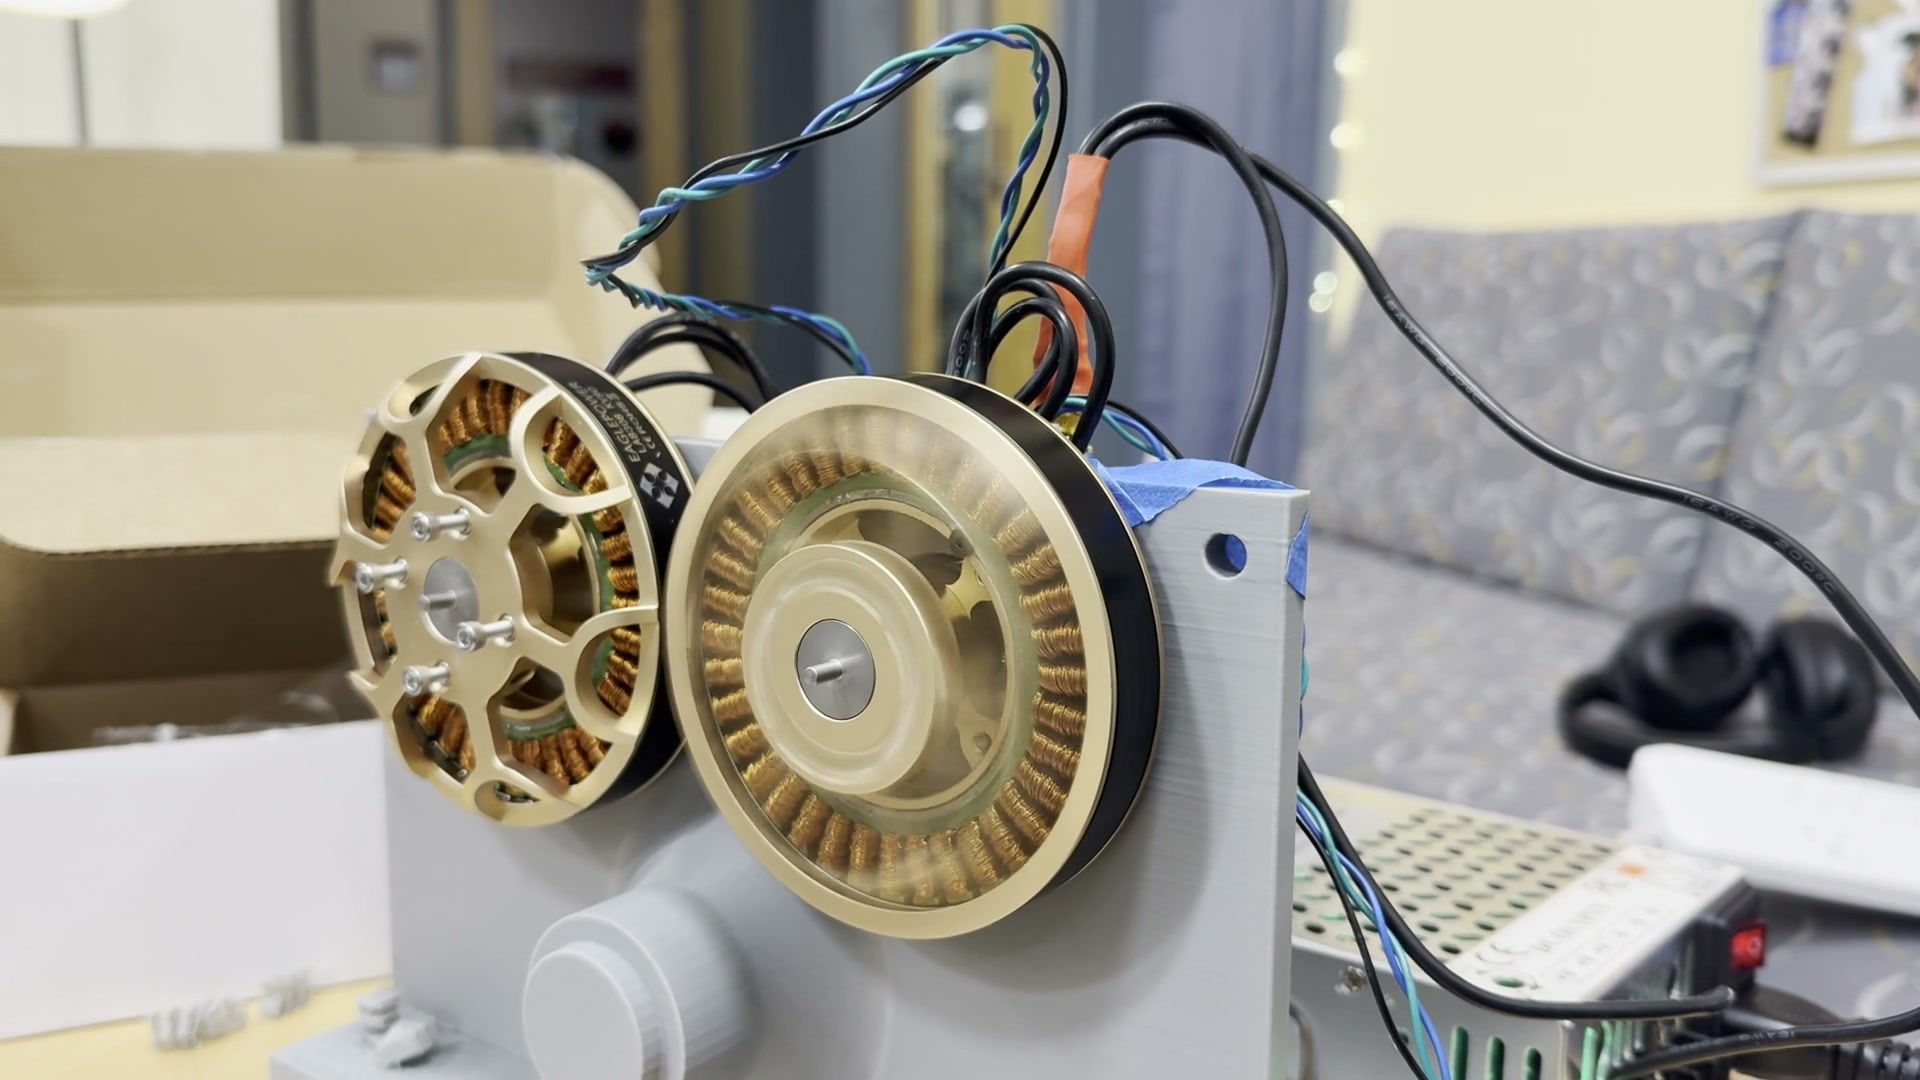
\includegraphics[width=\linewidth]{spin_blur2.jpg}
    \caption{At speed.}
  \end{subfigure}
  \caption{Frames from the first successful rotation. The right motor, under
  closed-loop control, blurs as it spins while the left motor stays still.}
  \label{fig:spin}
\end{figure}

\subsection{Two-motor control}

Next I set up the two controllers on one CAN-FD bus with IDs~1 and~2, powered
in parallel from the \SI{24}{\volt} supply, and first checked them with
\texttt{tview}. I then wrote small Python scripts on top of the
\texttt{moteus} asyncio library. The main one, \texttt{dual\_pos.py}, takes
position targets for both motors (in turns), sends trajectory-limited position
commands (velocity \SI{0.8}{turn\per\second}, acceleration
\SI{2}{turn\per\second\squared}, torque limit \SI{2}{\newton\metre}) with a
watchdog timeout, and refreshes the command until each move finishes. Other
scripts cover sweeps, keyboard and arrow-key jogging, and linkage calibration.

\subsection{Hand test of the capstan stage}

Before running the drive under power, I wrapped a printed large drum and turned
it by hand (Figure~\ref{fig:hand}). The 8:1 reduction is easy to see: a small
movement of the large drum spins the motor rotor through a much larger angle.
The motion was smooth, with no noticeable backlash when reversing direction.

\begin{figure}[H]
  \centering
  \begin{subfigure}[b]{0.32\linewidth}
    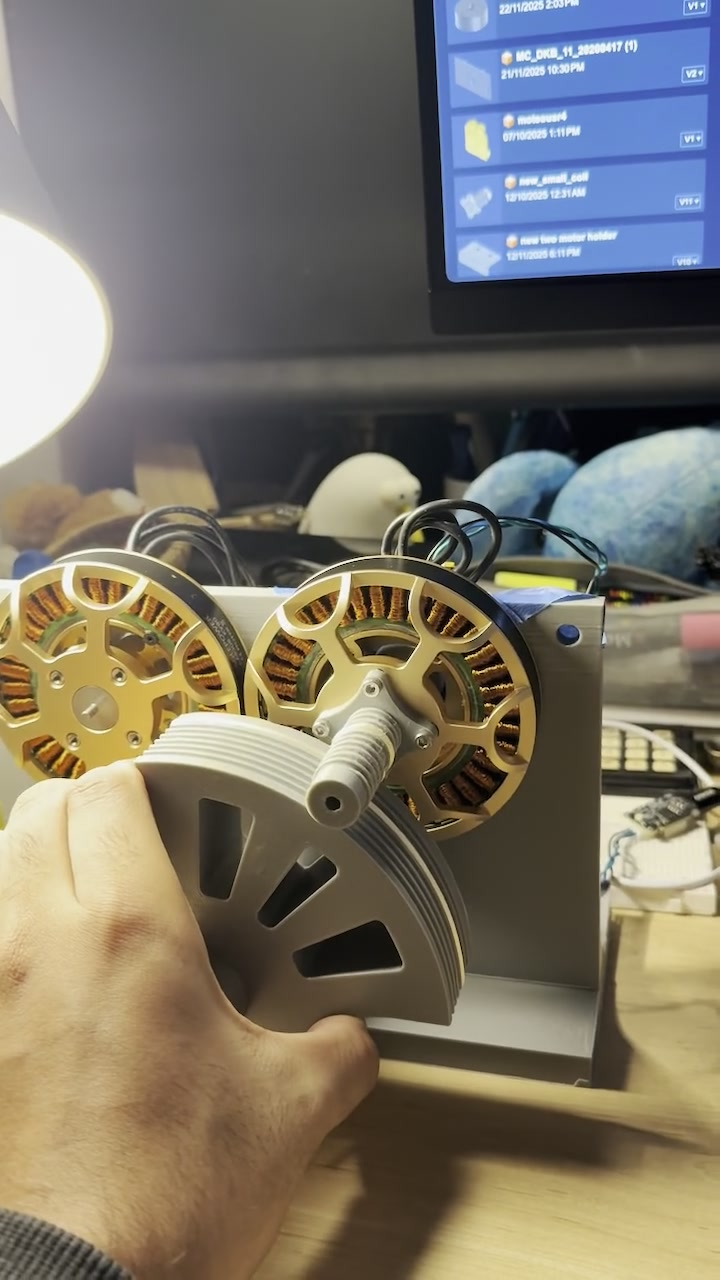
\includegraphics[width=\linewidth]{hand_a.jpg}
    \caption{}
  \end{subfigure}\hfill
  \begin{subfigure}[b]{0.32\linewidth}
    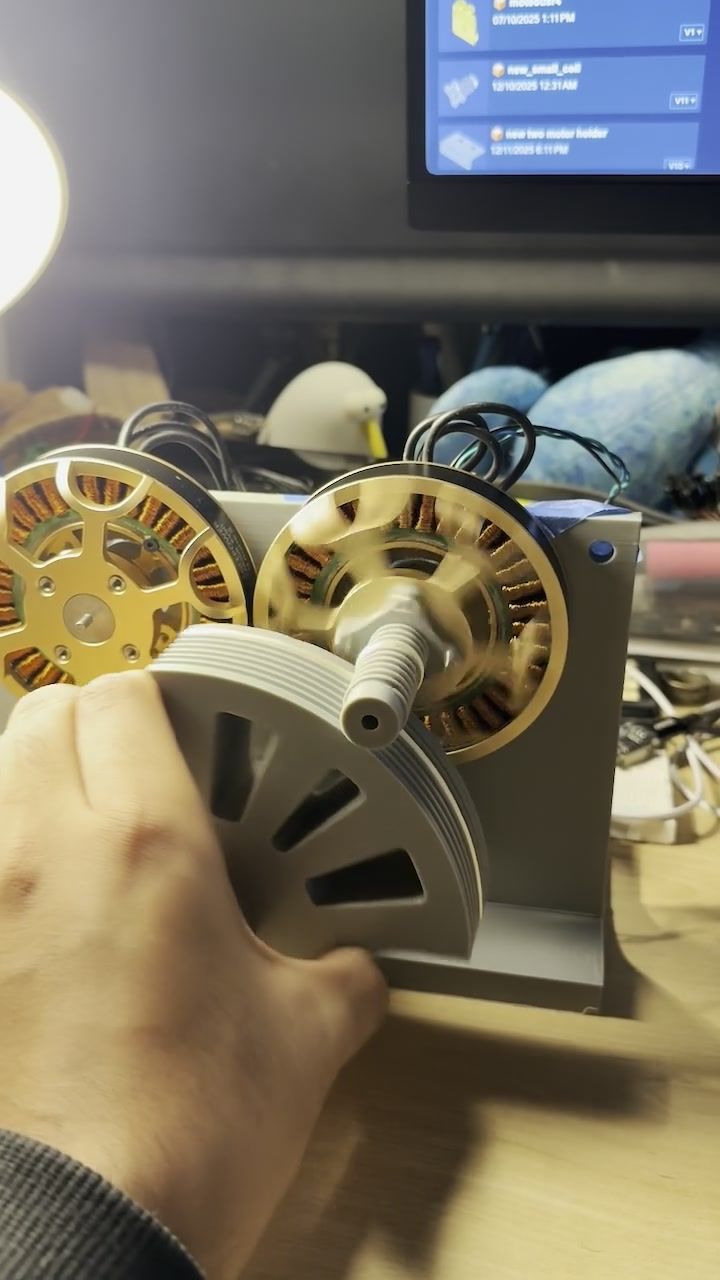
\includegraphics[width=\linewidth]{hand_b.jpg}
    \caption{}
  \end{subfigure}\hfill
  \begin{subfigure}[b]{0.32\linewidth}
    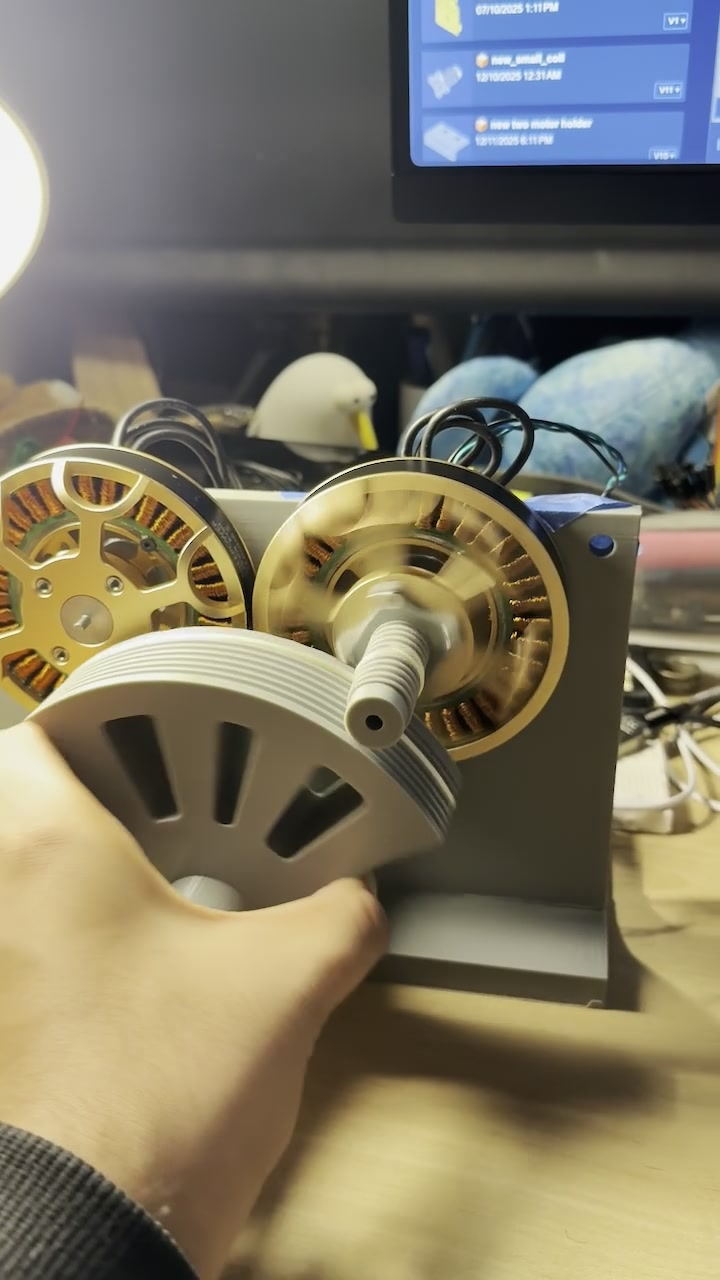
\includegraphics[width=\linewidth]{hand_c.jpg}
    \caption{}
  \end{subfigure}
  \caption{Back-driving the capstan stage by hand. The grooved large-drum
  sector turns about the output axle, and the rope drives the small threaded
  drum on the right-hand motor. Because the drive is back-drivable, the motor
  can be turned from the output side, which is what makes it suitable for
  force-sensitive legged control.}
  \label{fig:hand}
\end{figure}

% ===============================================================
\section{Lessons Learned}
% ===============================================================

\begin{itemize}
  \item \textbf{Check polarity before the first power-on.} Reversed supply leads
        nearly cost me a controller. I now check polarity with a multimeter and
        use keyed XT30 connectors throughout.
  \item \textbf{Use color-coded wire.} An all-black daisy-chain harness looked
        clean but caused a soldering mistake. Red/black power and colored CAN
        pairs are worth giving up the looks.
  \item \textbf{Ratio and wraps are separate design choices.} Diameters set the
        reduction; wraps set grip.
  \item \textbf{Mind the encoder air gap.} My first magnet holder put the magnet
        less than \SI{1}{\milli\metre} from the sensor, against a recommended
        gap of about \SI{2}{\milli\metre}. It worked, but it is being redesigned
        for reliable readings.
  \item \textbf{Confirm part dimensions on arrival.} One bearing order arrived
        in the wrong size and had to be returned, which held up assembly.
  \item \textbf{Ask the community.} The Moteus developer's help on Discord
        turned a stalled calibration into a working motor in an afternoon.
\end{itemize}

% ===============================================================
\section{Next Steps}
% ===============================================================

\begin{enumerate}
  \item Print the second motor's capstan drum and the main plate, then rope and
        tension both stages.
  \item Measure the real reduction ratio and adjust the large drum diameter to
        account for how much the rope flattens under tension.
  \item Redesign the encoder magnet holder for a \SI{2}{\milli\metre} gap.
  \item Characterize the drive: backlash, back-drive torque, torque ripple, and
        how much tension is lost over time.
  \item Attach the four-bar linkage and run the simulator's trajectories on
        hardware.
  \item Add the ab/adduction motor and move control onto a Raspberry Pi for an
        untethered 3-DOF leg, the first step toward a full quadruped.
\end{enumerate}

% ===============================================================
\section*{Acknowledgments}
% ===============================================================

Thank you to the BDW Makers Grant for funding this project, to Aaed Musa and the
Stanley quadruped project for publishing their designs openly, and to Josh
Pieper of mjbots for his help with Moteus configuration.

\section*{References}
\begin{enumerate}[label={[\arabic*]}]
  \item A.~Musa, ``Capstan Drive,''
        \url{https://www.aaedmusa.com/projects/capstandrive}.
  \item ``Stanley: The Capstan-Based Quadruped Kit,'' Hackaday.io,
        \url{https://hackaday.io/project/176726}.
  \item mjbots, ``Moteus r4.11 Reference Manual,''
        \url{https://github.com/mjbots/moteus}.
  \item ``Four-bar linkage,'' Wikipedia,
        \url{https://en.wikipedia.org/wiki/Four-bar_linkage}.
\end{enumerate}

\end{document}
